\documentclass[11pt,a4paper]{article}

\usepackage[T1]{fontenc}
\usepackage[utf8]{inputenc}
\usepackage{lmodern}
\usepackage[margin=0.88in,top=0.92in,bottom=0.92in]{geometry}
\usepackage{amsmath,amssymb,amsthm}
\usepackage{booktabs}
\usepackage{array}
\usepackage{graphicx}
\usepackage{float}
\usepackage{xcolor}
\usepackage{enumitem}
\usepackage[hidelinks]{hyperref}

\graphicspath{{figures/}}

\definecolor{accentblue}{HTML}{0F4C81}
\definecolor{slateink}{HTML}{334155}
\definecolor{softbg}{HTML}{F8FAFC}
\definecolor{ruleline}{HTML}{CBD5E1}

\hypersetup{
    colorlinks=true,
    linkcolor=accentblue,
    citecolor=accentblue,
    urlcolor=accentblue,
    pdftitle={DMCN and PDNC: Stateful Dendritic Neurons and Local Backpropagation-Free Learning for Non-Stationary Continual Tasks},
    pdfauthor={Shivam}
}

\newtheorem{proposition}{Proposition}

\setlength{\parskip}{0.45em}
\setlength{\parindent}{0pt}
\emergencystretch=1.8em
\setlist[itemize]{nosep,leftmargin=1.35em,itemsep=0.25em}
\setlist[enumerate]{nosep,leftmargin=1.45em,itemsep=0.25em}

\pagestyle{myheadings}
\markright{\small\itshape Preprint --- DMCN \& PDNC (For Peer Review)}

\title{\vspace{-1.0em}\Large\bfseries DMCN and PDNC: Stateful Dendritic Neurons and Local Backpropagation-Free Learning for Non-Stationary Continual Tasks}

\author{Shivam \\[0.25em]
\small\texttt{[Affiliation / ORCID / Contact Placeholder]} \\[0.15em]
\small\textit{Preprint --- Prepared for Peer Review (November 2026)}}
\date{}

\begin{document}
\maketitle
\thispagestyle{empty}

\begin{abstract}
\noindent Standard artificial neural networks rely on stateless point neurons, $y = \phi(Wx + b)$, trained end-to-end by global backpropagation. That design excels at offline optimization and large-scale pretraining, and this work does \textbf{not} claim to replace backpropagation on frontier vision or language models. Instead, we study the complementary regime where standard networks routinely fail: online streams in which inputs arrive sequentially across blank distractor delays, sensor amplitudes jump abruptly by $50\times$ to $100\times$, and new classes appear incrementally with \textbf{no replay buffer and no task labels}.

To clarify the division of labor between neuron design and multi-layer credit assignment, we separate two contributions and evaluate every claim under pre-registered, single-pass frozen protocols across $n = 20$ held-out random seeds (\texttt{2000--2019}) with matched baselines and null controls:
\textbf{(1)~DMCN} (\textit{Dendritic Multiplexed Cascade Neuron}) is a \textbf{stateful, multi-compartment neuron and layer architecture} combining causal divisive gain control, complex oscillating spine memory traces, active/bilinear dendritic branches, and orthogonal precision-matrix (or Gram--Cholesky) updates.
\textbf{(2)~PDNC} (\textit{Prospective Dendritic Natural-Credit}) is a \textbf{local, backpropagation-free and weight-transport-free multi-layer training algorithm} combining symmetric Kolen--Pollack feedback alignment, two-pass prospective settling, local metric conditioning, episode-rate eligibility traces, and overlapping local spatial patches.

Across streaming \texttt{Split-MNIST} corrupted by $4$ blank delay ticks and $50\times$ sensor gain jumps, DMCN reaches \textbf{$90.32\% \pm 0.06\%$} ($97.77\%$ Pair-0 retention, $0$ replay), still beating \texttt{Pooled ACIL} ($\mathbf{+21.64\text{ pp}}$) and \texttt{GRU + ER-200} ($\mathbf{+59.41\text{ pp}}$) even when both baselines receive DMCN's own causal gain normalizer. On 10-task RGB \texttt{Split-CIFAR-100} over frozen \texttt{MobileNetV2} embeddings ($0$ replay, $0$ task IDs), single-pass DMCN hits \textbf{$68.65\% \pm 0.09\%$}, matching the offline joint FP64 ridge bound within $0.0035\%$ while outperforming 10-epoch \texttt{MLP + ER-500} ($33.54\%$) by $+35.10\text{ pp}$. Replacing per-batch Woodbury inversions with checkpointed \textbf{Gram--Cholesky} solves speeds up GPU execution \textbf{$3.86\times$} on \texttt{Split-MNIST} ($81{,}936$ samples/s) and \textbf{$2.62\times$} on \texttt{Split-CIFAR-100} ($2.58\text{ s}$), while \textbf{$95\%$ sparse ternary} encoders preserve $68.65\%$ accuracy with $20\times$ fewer Layer-1 nonzeros. Causal Hedge self-gating resolves conflicting chaotic ($0.0054$ Lorenz NMSE) and $100\times$ shock ($0.0928$) regimes automatically, and sparse bilinear branches reach \textbf{$99.58\%$} zero-shot accuracy on unseen \texttt{Rule $\times$ Operand} compositions (vs.\ $83.75\%$ Backprop Adam).

At the same time, our experiments mark honest boundaries where local learning still falls short. On raw $16\times 16$ Pixel Pong RL, unsupervised Motion-Oja Layer-1 training failed ($39.05\%$ vs.\ $45.30\%$ frozen), locking onto bright static paddles instead of the ball. Adding \texttt{PDNC} over $4\times 4$ overlapping patches ($4{,}851$ L1 synapses, $13.5\times$ fewer than flat) lifts Pixel Pong to \textbf{$72.25\% \pm 4.68\%$}, tying Flat Backprop A2C ($72.30\%$) and beating Patch Backprop A2C ($68.90\%$), yet falls $1.75\text{ pp}$ short of our pre-registered $74.0\%$ target, shows wider cross-seed variance ($\text{SD} = 10.69\%$), and loses continual accuracy when hidden Layer-1 drift stales readout curvature on compact \texttt{Split-FashionMNIST} ($70.13\%$ plastic vs.\ $80.72\%$ frozen).
\end{abstract}

\noindent\textbf{Keywords:} dendritic neuron architecture, local plasticity, backpropagation-free learning, replay-free continual learning, causal gain control, resonant spine memory, Gram--Cholesky, sparse ternary weights, Kolen--Pollack feedback alignment, prospective dendritic natural-credit (\texttt{PDNC}).

\vspace{0.3em}\hrule\vspace{0.5em}

\section{Introduction}

Standard artificial neurons simplify biological computation down to a static dot product followed by a fixed nonlinearity. That abstraction has driven remarkable progress on offline deep learning. Yet the moment a deployed system must operate on real-time sensory streams---where inputs arrive over empty gaps, sensor scale fluctuates abruptly, and new categories appear one after another without storing past data---three distinct failure modes collide:
\begin{enumerate}
    \item \textbf{Amplitude fragility:} A sudden $50\times$ or $100\times$ jump in input gain pushes unnormalized sums into saturation and corrupts learned linear readouts. Online systems cannot peek at future frames to compute batch statistics.
    \item \textbf{Temporal amnesia:} Stateless layers forget cues from a few ticks earlier, whereas standard gradient-trained RNNs suffer severe catastrophic forgetting under sequential continual training without replay.
    \item \textbf{Catastrophic overwriting and weight transport:} Gradient descent overwrites prior tasks when shared weights shift without exemplars, while backpropagation demands symmetric weight transport ($W^\top$) along feedback pathways.
\end{enumerate}

Existing continual-learning methods typically resolve one piece in isolation. Regularization (\texttt{EWC}; Kirkpatrick et al., 2017) requires task boundaries; Experience Replay (\texttt{ER}; Chaudhry et al., 2019) buffers raw examples; and closed-form analytic learners (\texttt{ACIL}, Zhuang et al., 2022; \texttt{RanPAC}, McDonnell et al., 2023) execute exact sequential ridge regression over frozen projections on static, fixed-scale embeddings. Neither addresses simultaneous blank delays, causal scale shocks, autonomous pathway weighting, and backpropagation-free hidden feature training inside a unified framework.

\subsection{Clarifying DMCN and PDNC: Architecture vs.\ Training Algorithm}
Because local-learning proposals often blur neuron geometry with optimization rules, we define the exact boundary between our two contributions upfront:
\begin{itemize}
    \item \textbf{What is DMCN?} \textbf{DMCN} (\textit{Dendritic Multiplexed Cascade Neuron}) is a \textbf{new stateful, multi-compartment neuron and layer architecture}. Rather than collapsing each unit into $y = \phi(Wx+b)$, a DMCN layer integrates four local biophysical circuits: (1)~causal divisive gain control for positive scale invariance, (2)~damped complex oscillating spines that encode stimulus age in phase using fixed memory, (3)~active non-monotonic, self-gated, or bilinear dendritic branches, and (4)~local inverse-covariance (Woodbury or checkpointed Gram--Cholesky) updates that confine new learning to orthogonal directions.
    \item \textbf{What is PDNC?} \textbf{PDNC} (\textit{Prospective Dendritic Natural-Credit}) is a \textbf{new local, back\-propagation-free multi-layer training algorithm}. When DMCN sits over fixed dendritic expansions or pretrained features, only the readout adapts analytically. Whenever hidden Layer-1 weights must themselves be learned from raw pixels or noisy coordinates without \texttt{.backward()} or weight transport, \texttt{PDNC} drives hidden plasticity via symmetric Kolen--Pollack feedback alignment, two-pass prospective settling, local metric conditioning, and episode-rate three-factor eligibility traces (optionally structured into overlapping $4\times 4$ patches).
    \item \textbf{Where are PDNC's boundaries?} \texttt{PDNC} is a working local training rule, not a drop-in substitute for deep end-to-end backprop. Our tests expose two clear limits: continuous Layer-1 feature drift degrades closed-form continual readouts on compact \texttt{Split-FashionMNIST} ($70.13\%$ plastic vs.\ $80.72\%$ frozen), and sparse-reward pixel RL exhibits wider cross-seed spread ($\text{SD} = 10.69\%$) than Backprop A2C ($\text{SD} = 6.97\%$).
\end{itemize}

\subsection{Scope and Contributions}
DMCN and PDNC target online single-pass continual learning under gain shocks and delays, zero-shot rule binding, transport-free visual policy learning, and compact decentralized control. They do \textbf{not} replace backpropagation for pretraining large vision backbones (our \texttt{Split-CIFAR-100} benchmark uses frozen \texttt{MobileNetV2} embeddings) or large language models. Our main contributions are:
\begin{enumerate}
    \item \textbf{Unified 4-Pillar Neuron Circuit (\texttt{DMCN}):} Integrates causal divisive homeostasis (Proposition~1), complex Zero-Order-Hold spine oscillators ($O(K d_{\text{in}})$ memory), active/bilinear/self-gated dendrites, and batch-order-invariant Woodbury / Gram--Cholesky plasticity (Proposition~2).
    \item \textbf{Fairness-Controlled Benchmarks:} Demonstrates that even when \texttt{Pooled ACIL} and \texttt{GRU + ER-200} are handed DMCN's own causal gain normalizer, DMCN retains $+21.64\text{ pp}$ and $+59.41\text{ pp}$ leads on streaming delayed-cue + $50\times$ shock \texttt{Split-MNIST}, and matches offline FP64 ridge regression within $0.0035\%$ on 100-class RGB \texttt{Split-CIFAR-100}.
    \item \textbf{GPU Speed and $95\%$ Sparsity:} Eliminates per-batch Woodbury inversions via checkpointed \textbf{Gram--Cholesky} solves ($3.86\times$ speedup on \texttt{Split-MNIST}, $2.62\times$ on \texttt{Split-CIFAR-100}) paired with $95\%$ sparse ternary $\{-1, 0, +1\}$ encoders ($20\times$ fewer L1 nonzeros, $0\%$ accuracy loss) and $3.99\times$ precision-RAM savings via 4-branch block-diagonal partitioning.
    \item \textbf{Autonomous Self-Gating \& Zero-Shot Composition:} Resolves opposing Lorenz chaos ($0.0054$ NMSE) and $100\times$ gain-shock ($0.0928$) tasks under one frozen config, and reaches $99.58\%$ zero-shot \texttt{Rule $\times$ Operand} generalization via competitive Oja + bilinear branches.
    \item \textbf{Local Visual Credit (\texttt{PDNC}) and Failure Mapping:} Ties Flat Backprop A2C on raw $16\times 16$ Pixel Pong ($72.25\%$ vs.\ $72.30\%$) using $4\times 4$ local patches ($4{,}851$ L1 synapses vs.\ $65{,}536$), while transparently documenting the refuted unsupervised Motion-Oja hypothesis ($39.05\%$) and continual L1 drift conflict.
\end{enumerate}

\section{Background and Related Work}

Biological pyramidal neurons compute nonlinear functions locally along dendritic branches via NMDA plateaus, calcium spikes (Larkum, 2013), and human cortical dendritic calcium action potentials (\texttt{dCaAPs}; Gidon et al., 2020; Poirazi et al., 2003). DMCN abstracts this compartmental separation into smooth non-monotonic gates and pairwise branch multiplication.

In continual learning, \texttt{EWC} (Kirkpatrick et al., 2017) requires known task boundaries and falters under class-incremental streaming (van de Ven \& Tolias, 2019), while \texttt{ER} (Chaudhry et al., 2019) stores past inputs and cascade models (Benna \& Fusi, 2016) consolidate across coupled timescales. Analytic continual learners (\texttt{ACIL}, Zhuang et al., 2022; \texttt{RanPAC}, McDonnell et al., 2023) use recursive least squares over frozen features to match offline ridge solutions in one pass. Our controlled baselines verify that on static embeddings DMCN reduces to exact RLS over a skip-augmented dendritic basis, whereas under temporal delays and gain shocks, static and pooled ACIL degrade without causal homeostasis and complex spines.

For temporal state spaces and local credit assignment, DMCN's spine bank echoes Legendre Memory Units (\texttt{LMU}; Voelker \& Eliasmith, 2018) in simplified diagonal complex form ($O(K d_{\text{in}})$ state), while \texttt{PDNC} unifies symmetric Kolen--Pollack feedback alignment (Kolen \& Pollack, 1994; Akrout et al., 2019)---overcoming fixed random Feedback Alignment (Lillicrap et al., 2016)---with two-sweep prospective configuration (Song et al., 2024).

\begin{table}[htbp]
\centering
\caption{Structural Comparison Across Neural Learning Paradigms.}
\label{tab:paradigms}
\small
\resizebox{\linewidth}{!}{%
\begin{tabular}{@{}lllll@{}}
\toprule
\textbf{Property} & \textbf{Point MLP + Adam/EWC} & \textbf{GRU + ER-200} & \textbf{ACIL / RanPAC} & \textbf{DMCN / PDNC (Ours)} \\
\midrule
Zero \texttt{.backward()} / Zero Weight Transport & No & No & Readout only & \textbf{Yes (100\% local)} \\
Replay-Free, Task-ID-Free CL & Fails ($9\text{--}20\%$) & Needs buffer & Yes (static) & \textbf{Yes ($95.8\%$ MNIST, $68.7\%$ C100)} \\
Causal Gain-Shock Invariance ($50\times\text{--}100\times$) & No & No & No & \textbf{Yes (Prop.\ 1: Causal RMS)} \\
Temporal Order Across Blank Delays & No & BPTT (forgets CL) & Pooled fails ($68.7\%$) & \textbf{Yes ($90.3\%$ complex spines)} \\
Zero-Shot \texttt{Rule $\times$ Operand} Binding & Partial ($83.8\%$) & --- & Linear only & \textbf{Yes ($99.6\%$ Oja + Bilinear)} \\
Multi-Layer Raw-Pixel RL ($0$ \texttt{.backward()}) & Backprop & Backprop & Frozen L1 ($30.5\%$) & \textbf{Yes ($72.3\%$ Patch PDNC)} \\
\bottomrule
\end{tabular}}
\end{table}

\section{The DMCN Neuron Architecture}

Rather than evaluating one stateless dot product per unit, each DMCN layer operates a compact local control circuit (Figure~\ref{fig:arch}A, Table~\ref{tab:state}): causal gain normalization stabilizes amplitude, complex spine oscillators preserve timing, active/bilinear dendritic compartments shape local nonlinearities, and orthogonal second-order plasticity protects prior knowledge without replay.

\begin{figure}[htbp]
    \centering
    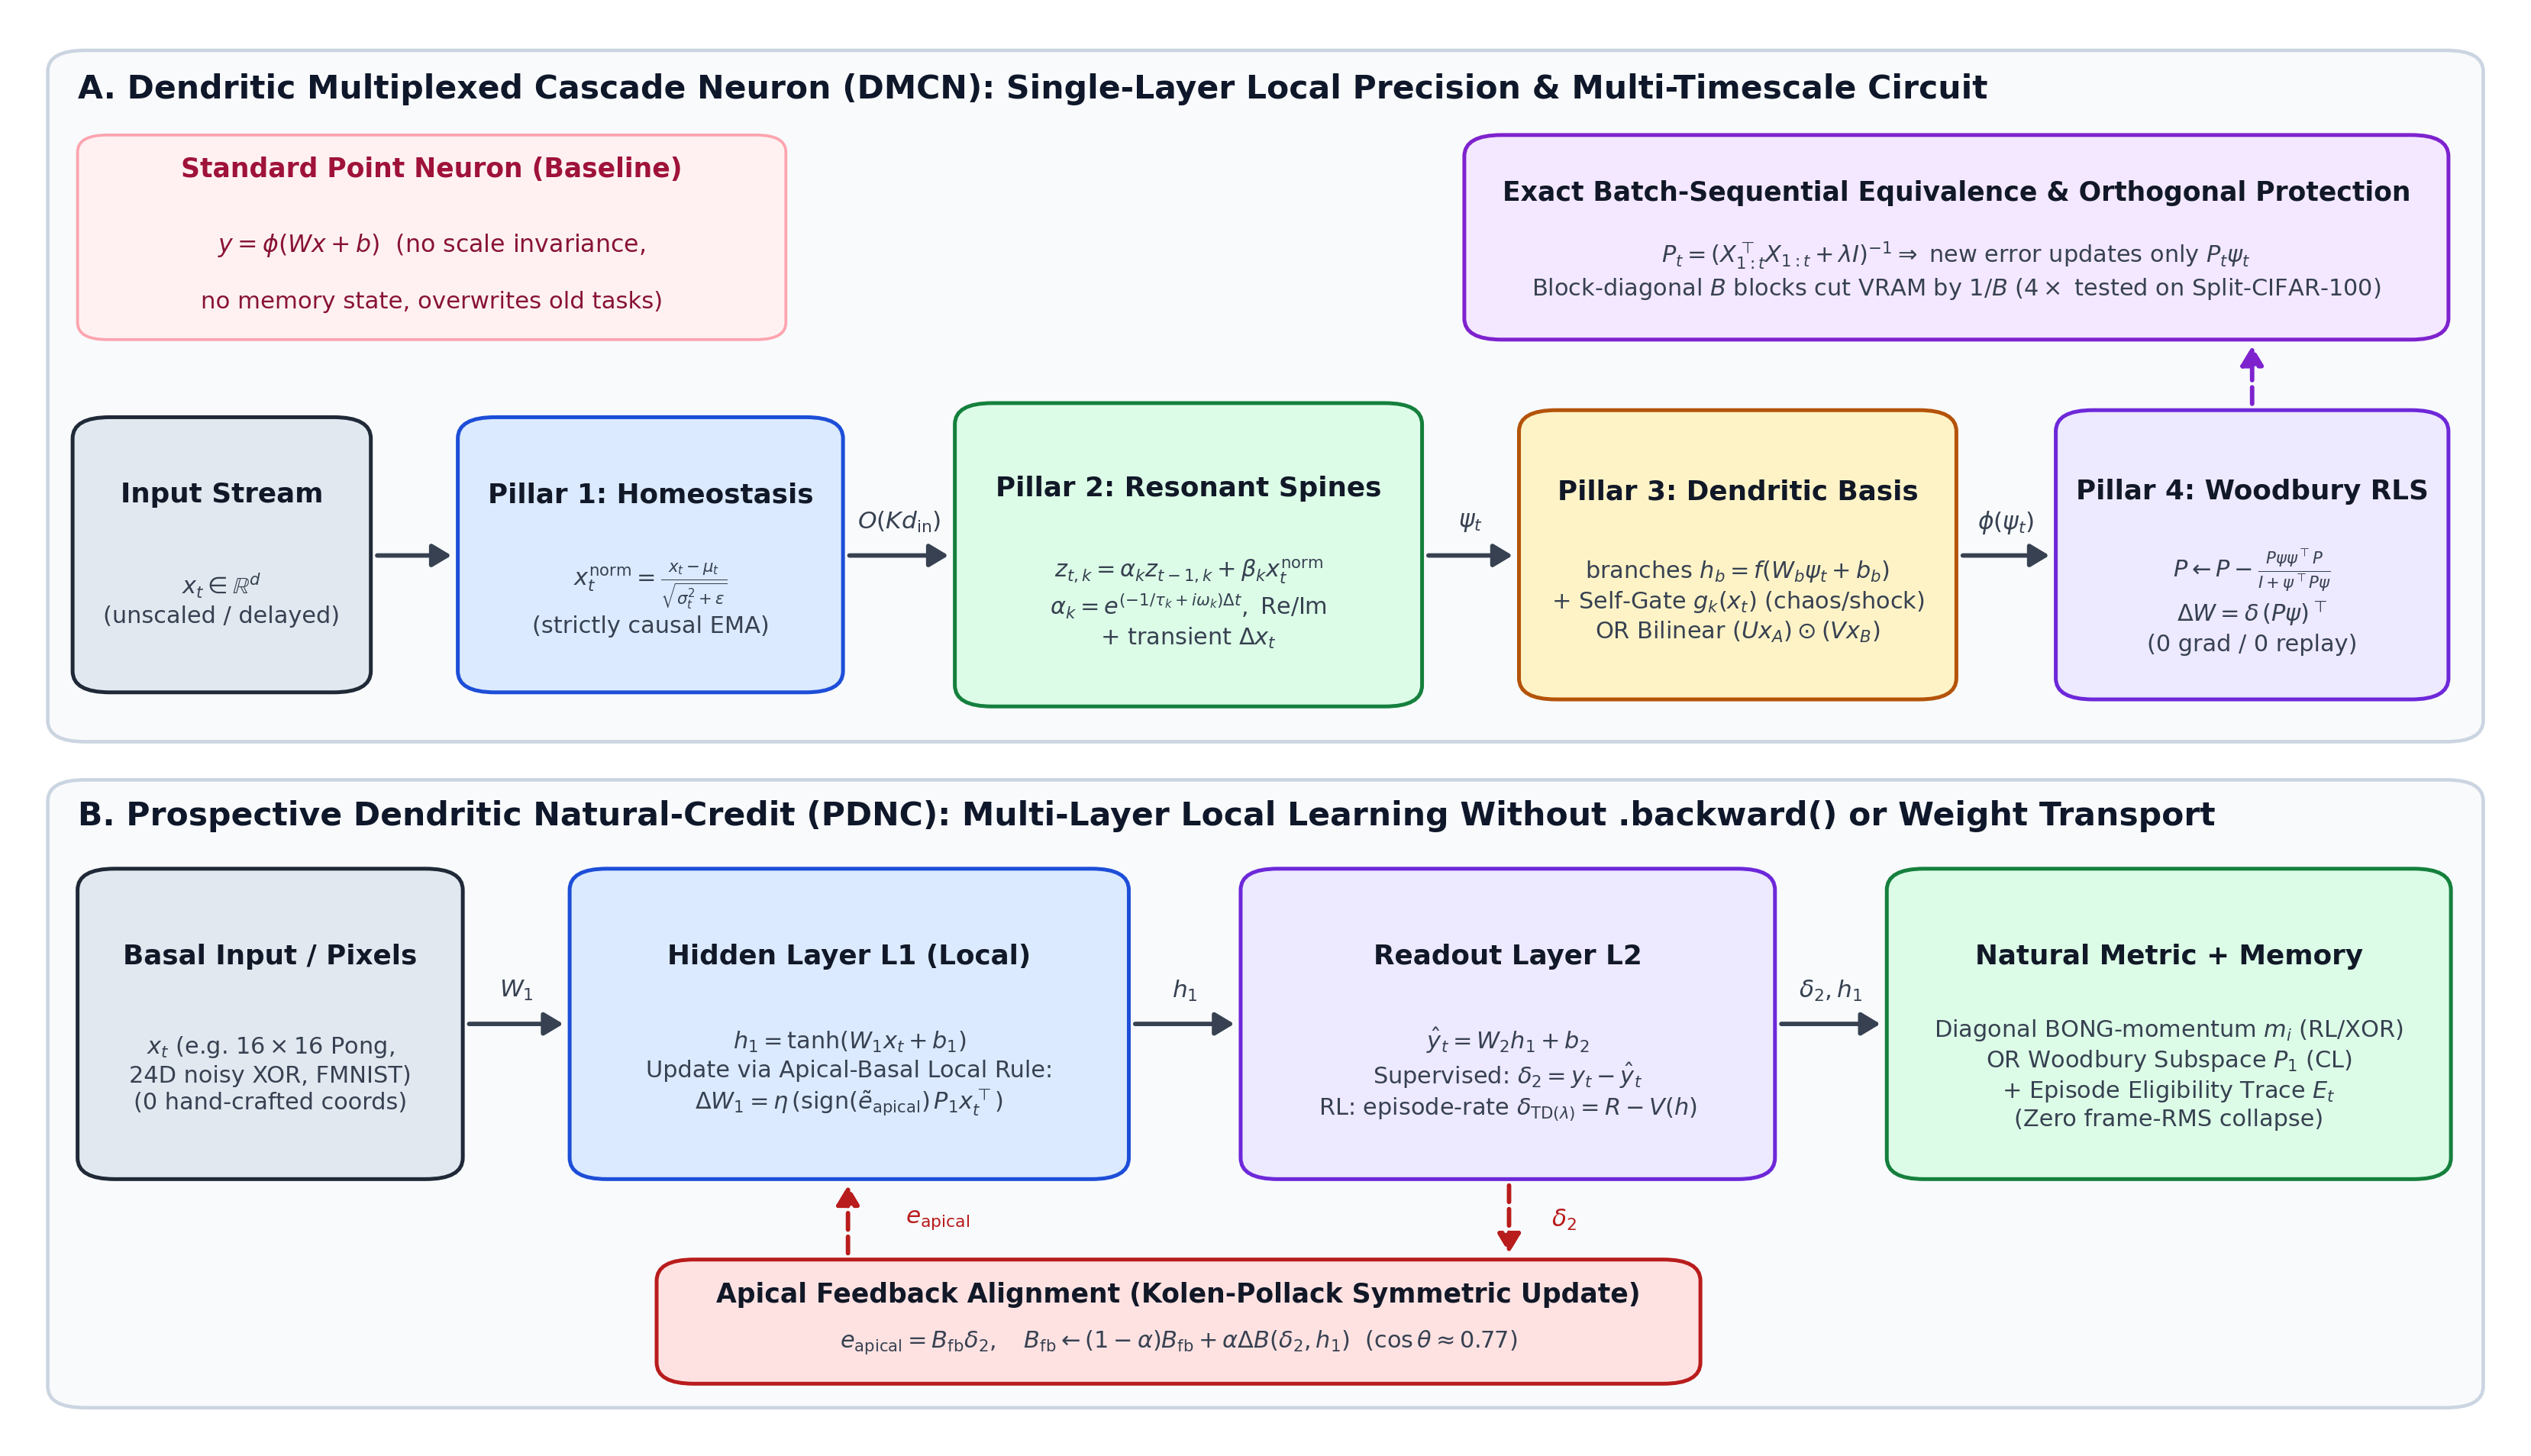
\includegraphics[width=0.98\linewidth]{fig0_dmcn_pdnc_architecture.png}
    \caption{Architecture and algorithm overview. \textbf{(A) DMCN:} Causal RMS gain control, complex ZOH spine oscillators ($O(K d_{\text{in}})$ memory), active/self-gated/bilinear dendrites, and Woodbury or checkpointed Gram--Cholesky plasticity. \textbf{(B) PDNC:} Backpropagation-free hidden-layer training via disjoint Kolen--Pollack feedback ($B_{\text{fb}} \to W^\top$), prospective settling, local metric conditioning, and episode-rate TD($\lambda$) traces.}
    \label{fig:arch}
\end{figure}

\begin{table}[htbp]
\centering
\caption{Persistent Internal State and Memory Complexity of a Single DMCN / PDNC Layer.}
\label{tab:state}
\small
\resizebox{\linewidth}{!}{%
\begin{tabular}{@{}llll@{}}
\toprule
\textbf{State / Tensor} & \textbf{Shape} & \textbf{Role} & \textbf{Memory Complexity} \\
\midrule
Causal energy $e_t$ (or $\bar{\sigma}^2_t$) & Scalar or $(d_{\text{in}},)$ & Strictly causal divisive RMS normalizer & $O(d_{\text{in}})$ \\
Resonant spine state $z_k[t]$ & $(K, d_{\text{in}})$ & ZOH complex oscillator bank & $O(K d_{\text{in}})$, constant in stream $T$ \\
Dendritic weights $W_{\text{slow}}, W_{\text{fast}}, W_{\text{eff}}$ & $(B, d_{\text{out}}, d_\psi)$ & Multi-timescale branch synaptic weights & $O(B\, d_{\text{out}}\, d_\psi)$ \\
Surprise prototypes $C$ & $(B, d_\psi)$ & Branch context keys & $O(B\, d_\psi)$ \\
Precision $P$ or Gram $(G, H)$ & $(d_\psi, d_\psi)$, $(d_\psi, d_{\text{out}})$ & Orthogonal subspace memory & $O(d_\psi^2)$ ($O(d_\psi^2/B_{\text{diag}})$ block-diag) \\
Apical feedback $B_{\text{fb}}$ & $(d_{\text{in}}, d_{\text{out}})$ & Kolen--Pollack feedback matrix & $O(d_{\text{in}}\, d_{\text{out}})$ (disjoint RNG seed) \\
\bottomrule
\end{tabular}}
\end{table}

\subsection{Pillar 1: Causal Divisive Homeostasis}
In episodic streaming over $x_t \in \mathbb{R}^{d_{\text{in}}}$, DMCN tracks a strictly causal peak-energy envelope using only past and present samples:
\begin{equation}
e_0 = \frac{1}{d_{\text{in}}}\|x_0\|_2^2, \qquad
e_t = \max\!\left(0.98\, e_{t-1},\; \frac{1}{d_{\text{in}}}\|x_t\|_2^2\right), \qquad
\tilde{x}_t = \operatorname{clip}\!\left(\frac{x_t}{\sqrt{e_t + \epsilon}},\; -8,\; 8\right).
\end{equation}
In continuous stationary streams, it tracks a causal running variance updated after normalizing the incoming frame so future statistics never leak backward.

\begin{proposition}[Exact Positive Gain-Shock Invariance]
For any sequence $x_{0:T}$ and positive scale factor $g > 0$ ($x'_t = g x_t$), the causal envelope obeys $e_t(gx) = g^2 e_t(x)$ for all $t \ge 0$. Whenever $g^2 e_t(x) \gg \epsilon$, the normalized stream satisfies $\tilde{x}'_t = \tilde{x}_t$ identically using strictly causal operations.
\end{proposition}
\begin{proof}
At $t=0$, $e_0(gx) = \frac{1}{d_{\text{in}}}\|gx_0\|_2^2 = g^2 e_0(x)$. Assuming $e_{t-1}(gx) = g^2 e_{t-1}(x)$, since $\max(ag^2, bg^2) = g^2\max(a,b)$ for $g > 0$, we obtain $e_t(gx) = g^2 e_t(x)$ at step $t$. Dividing $gx_t$ by $\sqrt{g^2 e_t(x)+\epsilon}$ cancels $g$ at every step by induction.
\end{proof}

\subsection{Pillar 2: Resonant Complex Spine Oscillators}
Real decaying traces blur multi-step sequences delivered before blank pauses into an unordered average. DMCN instead attaches $K$ uncoupled damped complex oscillators, $\dot{z}_k = (-1/\tau_k + i\omega_k)z_k + \frac{1}{\tau_k}\tilde{x}_t$, integrated via exact Zero-Order Hold ($\Delta t = 1$, $r_k = e^{-1/\tau_k}$):
\begin{equation}
z_k[t] = r_k e^{i\omega_k}\, z_k[t-1] + (1 - r_k)\,\tilde{x}_t, \qquad k = 1, \dots, K,
\end{equation}
forming the composite representation
\begin{equation}
\psi_t = \left[\tilde{x}_t,\; \operatorname{Re}(z_1[t]), \dots, \operatorname{Re}(z_K[t]),\; \operatorname{Im}(z_1[t]), \dots, \operatorname{Im}(z_K[t])\right] \in \mathbb{R}^{(2K+1)d_{\text{in}}}.
\end{equation}
Because a stimulus arriving $m$ steps earlier rotates by phase angle $m\omega_k$, distinct temporal positions become linearly separable cosine-sine patterns at readout time $T$ in fixed $O(K d_{\text{in}})$ state.

\subsection{Pillar 3 \& 4: Active Dendrites, Orthogonal Plasticity, and GPU Acceleration}
For compartment $b \in \{1,\dots,B\}$ with drive $u_b = W_b^{\text{eff}}\psi_t - \theta_b$, DMCN combines $\tanh(u_b)$ with a smooth dCaAP-style band-pass gate (Gidon et al., 2020), $\phi_{\text{dend}}(u_b) = (1-\rho_b)\tanh(u_b) + \rho_b(\sigma(\beta(u_b-\vartheta_{\text{on},b})) - \sigma(\beta(u_b-\vartheta_{\text{off},b})))$ with $\vartheta_{\text{off},b} > \vartheta_{\text{on},b}$, enabling single-layer XOR separation.

To learn sequential tasks without replay, the readout initializes an inverse-covariance matrix $P_0 = \lambda^{-1} I$. Given mini-batch $X_t \in \mathbb{R}^{B \times d}$ and residual $E_t = Y_t - X_t W_{t-1}^\top$, exact Woodbury updates confine weight changes primarily to unused subspace axes:
\begin{align}
K_t &= P_{t-1} X_t^\top, \qquad S_t = I_B + X_t K_t, \qquad G_t = (S_t^{-1} K_t^\top)^\top, \\
W_t &= W_{t-1} + E_t^\top G_t^\top, \qquad P_t = \tfrac{1}{2}\!\left[(P_{t-1} - G_t K_t^\top) + (P_{t-1} - G_t K_t^\top)^\top\right].
\end{align}

\begin{proposition}[Exact Batch-Sequential Equivalence]
For any mini-batch partition of $\mathbf{X}_{1:T}$ ($B \ge 1$), exact Woodbury updates maintain $P_t = (\mathbf{X}_{1:t}^\top\mathbf{X}_{1:t} + \lambda I)^{-1}$ and $W_t^\top = (\mathbf{X}_{1:t}^\top\mathbf{X}_{1:t} + \lambda I)^{-1}\mathbf{X}_{1:t}^\top \mathbf{Y}_{1:t}$, invariant to batch size and task order.
\end{proposition}
\begin{proof}
By the matrix inversion lemma on $P_t^{-1} = P_{t-1}^{-1} + X_t^\top X_t$, $P_t = P_{t-1} - G_t K_t^\top$ and $P_t X_t^\top = G_t$. Multiplying $W_t^\top = W_{t-1}^\top + G_t(Y_t - X_t W_{t-1}^\top)$ on the left by $P_t^{-1}$ yields $(P_{t-1}^{-1} + X_t^\top X_t)W_{t-1}^\top + X_t^\top(Y_t - X_t W_{t-1}^\top) = \mathbf{X}_{1:t-1}^\top\mathbf{Y}_{1:t-1} + X_t^\top Y_t = \mathbf{X}_{1:t}^\top\mathbf{Y}_{1:t}$.
\end{proof}

\textbf{GPU Acceleration and Sparsity.} Solving $S_t^{-1}$ every mini-batch costs $O(B d^2 + B^3)$ per step. We remove this bottleneck without altering the mathematics:
\begin{enumerate}
    \item \textbf{Block-Diagonal Branches:} Partitioning dendrites into $B_{\text{diag}}$ independent branches cuts precision storage by $1/B_{\text{diag}}$ ($16.79\text{ MB} \to 4.21\text{ MB}$ at $B_{\text{diag}}=4$, $3.99\times$ reduction).
    \item \textbf{Checkpointed Gram--Cholesky + $95\%$ Sparse Ternary Encoders:} Accumulating normal equations $G \mathrel{+}= X_t^\top X_t$ (from $\lambda I$) and $H \mathrel{+}= X_t^\top Y_t$ during streaming and running one Cholesky solve $W^\top = G^{-1}H$ at evaluation checkpoints preserves Proposition~2 identically while achieving $2.62\times\text{--}3.86\times$ GPU speedups. Sampling Layer-1 projections with $95\%$ zeros in $\{-1, 0, +1\}$ cuts L1 nonzeros $20\times$ with zero accuracy drop (standard \texttt{torch.mm} still runs dense FP32 multiply-adds; physical sparsity speedups require custom bit-packed kernels).
\end{enumerate}

\noindent\fbox{\parbox{0.97\linewidth}{\small
\textbf{Algorithm 1: Single-Layer DMCN Forward and Local Plasticity Step (Zero \texttt{.backward()})}
\begin{enumerate}
    \item \textbf{Gain Control:} Update causal energy $e_t$ (or running variance); compute clipped $\tilde{x}_t$.
    \item \textbf{Spine Oscillators:} Step $z_k[t] = r_k e^{i\omega_k} z_k[t-1] + (1 - r_k)\tilde{x}_t$; assemble $\psi_t = [\tilde{x}_t, \operatorname{Re}(z), \operatorname{Im}(z)]$.
    \item \textbf{Dendrites:} Evaluate branch potentials $u_b$, apply $\phi_{\text{dend}}(u_b)$ (or self-gated/bilinear outputs), predict $y_t$.
    \item \textbf{Plasticity (when target present):} \textit{gram\_cholesky}: $G \mathrel{+}= \psi^\top\psi$, $H \mathrel{+}= \psi^\top Y$, solve Cholesky at checkpoints; \textit{woodbury}: update $W, P$ orthogonally; \textit{cascade}: normalized delta + Benna--Fusi tag consolidation.
\end{enumerate}
}}

\subsection{Autonomous Pathway Self-Gating and Bilinear Factorization}
To prevent manual tuning across incompatible tasks, a self-gating layer runs four parallel experts (\texttt{raw}, \texttt{homeo}, \texttt{spine}, \texttt{transient}) and weights them causally via Hedge exponential weights on each pathway's own smoothed prediction error $L_{t,m}$:
\begin{equation}
g_{t,m} \propto \exp\!\left(-\beta_{\text{gate}}\,\frac{L_{t,m} - \min_j L_{t,j}}{\bar{L}_t + \epsilon}\right).
\end{equation}
For compositional rule-operand binding, a factorized bilinear layer first extracts sparse factors $u \in \mathbb{R}^N$ via top-$k$ competitive Oja learning with homeostatic fatigue and soft $\ell_1$ shrinkage, $w_b \leftarrow \mathcal{S}_{\lambda_1}(w_b + \eta y_b(x_u - y_b w_b))$, before feeding $\tanh(1.5 u)$ alongside all $\binom{N}{2}$ pairwise products $u_i u_j$ ($i < j$) into ridge plasticity.

\section{The PDNC Multi-Layer Training Algorithm}

When lower hidden layers cannot remain frozen and must learn features from raw pixels or noisy dimensions without \texttt{.backward()} or weight transport, \textbf{PDNC} coordinates multi-layer plasticity through four local rules (Figure~\ref{fig:arch}B, Algorithm~2):
\begin{enumerate}
    \item \textbf{Disjoint Symmetric Kolen--Pollack Feedback:} Forward weights $W$ and apical feedback $B_{\text{fb}}$ initialize from independent RNG streams and update via matched local endpoint outer products plus decay so $B_{\text{fb}} \to W^\top$ organically (Kolen \& Pollack, 1994; Akrout et al., 2019).
    \item \textbf{Two-Pass Prospective Settling:} In supervised settings, lower layers settle and recompute post-update activations $h_\ell^{\text{settled}}$ before upper layers commit readout updates (Song et al., 2024).
    \item \textbf{Metric Conditioning (\texttt{diagonal} vs.\ \texttt{subspace}):} Stationary RL and noisy XOR use diagonal inverse second moments; boundary-free continual shifts use an online Woodbury subspace matrix $P_1$.
    \item \textbf{Episode-Rate Eligibility and $4\times 4$ Visual Patches (RL):} Actor and Critic apical signals sum at Layer-1 compartments to accumulate three-factor traces $E_W \leftarrow \gamma\lambda E_W + \delta_{\text{soma}}\psi^\top$, consolidated at episode end with zero replay buffer. On $16\times 16$ pixels, restricting compartments to overlapping $4\times 4$ patches (stride $2$, $3$ compartments/patch $\Rightarrow 147$ units, $4{,}851$ L1 synapses vs.\ $65{,}536$ flat; zero weight sharing, zero coordinates) curbs alignment variance.
\end{enumerate}

\noindent\fbox{\parbox{0.97\linewidth}{\small
\textbf{Algorithm 2: PDNC Multi-Layer Local Credit (Zero \texttt{.backward()}, Zero Weight Transport)}
\begin{itemize}
    \item \textbf{Supervised:} (1) Apical sweep $\delta_\ell = (B_{\text{fb},\ell+1}\delta_{\ell+1})\odot\phi'(u_\ell)$; (2) Update $W_\ell, B_{\text{fb},\ell}$ via diagonal or subspace conditioning and recompute settled $h_\ell = \phi(W_\ell \psi_\ell)$; (3) Update readout from settled error.
    \item \textbf{RL (No Replay):} Each tick $t$, sum Actor + Critic apical signals and accumulate $E_W \leftarrow \gamma\lambda E_W + \delta_{\text{soma},t}\psi_t^\top$; apply TD($\lambda$)-modulated consolidation at \texttt{done=True}.
\end{itemize}
}}

\textbf{Architectural Limit --- Hidden Drift vs.\ Readout Precision.} Updating Layer-1 weights shifts hidden feature coordinates $H = \phi(W_1 X)$. If a top continual readout holds an accumulated inverse curvature matrix $P_2 = (H_{\text{old}}^\top H_{\text{old}} + \lambda I)^{-1}$, subsequent Layer-1 drift invalidates $P_2$, causing forgetting relative to frozen L1 bases (Section~\ref{sec:pdnc_results}).

\section{Experimental Protocol}

All experiments were pre-registered prior to evaluation, tuned strictly on validation \texttt{seed 999} (from \texttt{[980..999]}), and executed once under frozen code across \textbf{$n = 20$ held-out test seeds (\texttt{2000--2019})}, reporting $\text{mean} \pm 95\%\text{ CI}$ ($1.96\,\text{SD}/\sqrt{20}$), SD, and min--max. Mandatory null controls (\texttt{Untrained}, \texttt{Blind} zeroed inputs, \texttt{Shuffled} labels/rewards, \texttt{Majority}, \texttt{Random}, \texttt{Decoupled}, \texttt{Scrambled}) accompany validation-tuned baselines (\texttt{ER-500}, \texttt{GRU + ER-200}, \texttt{Backprop A2C}, \texttt{PID Observer}). On \texttt{Split-CIFAR-100}, 1-epoch training left \texttt{MLP + ER-500} undertrained ($6.30\%$ on \texttt{seed 999}), so gradient baselines were tuned to $10$ epochs/task ($33.68\%$ val) and \texttt{Linear-RLS} to $\lambda = 1.0$ ($64.98\%$ val). GPU tests ran on an NVIDIA GeForce RTX 3060 (PyTorch \texttt{2.6.0+cu124}, Python \texttt{3.12.10}).

\section{Empirical Results}

\subsection{Simultaneous Time, \texorpdfstring{$50\times$}{50x} Gain Shocks, and Zero-Replay Continual Learning}
MNIST digits stream over $11$ ticks ($7$ noisy $112$-px horizontal strips + $4$ blank noise frames, classified at $t=10$) sequentially across $\{0,1\}\to\dots\to\{8,9\}$ with $0$ replay, $0$ task IDs, $50\times$ training gain jumps ($[1.0, 6.0, 0.2, 10.0, 0.4]$), and unseen test gains in $[0.2, 10.0]$. Intact DMCN reaches \textbf{$90.32\% \pm 0.06\%$} ($97.77\%$ Pair-0 retention), while removing any single pillar cuts accuracy by $50.4$ to $76.2\text{ pp}$ (Figure~\ref{fig:unified}, Table~\ref{tab:temporal}). Handing DMCN's \texttt{CausalRMS} normalizer directly to rivals raises \texttt{Pooled ACIL} to $68.66\%$ and \texttt{GRU + ER-200} to $30.88\%$, yet Unified DMCN ($90.30\%$ in the matched control suite) maintains $+21.64\text{ pp}$ and $+59.41\text{ pp}$ leads because pooled averages discard strip order across the blank delay (Figure~\ref{fig:controls}A).

\begin{figure}[htbp]
    \centering
    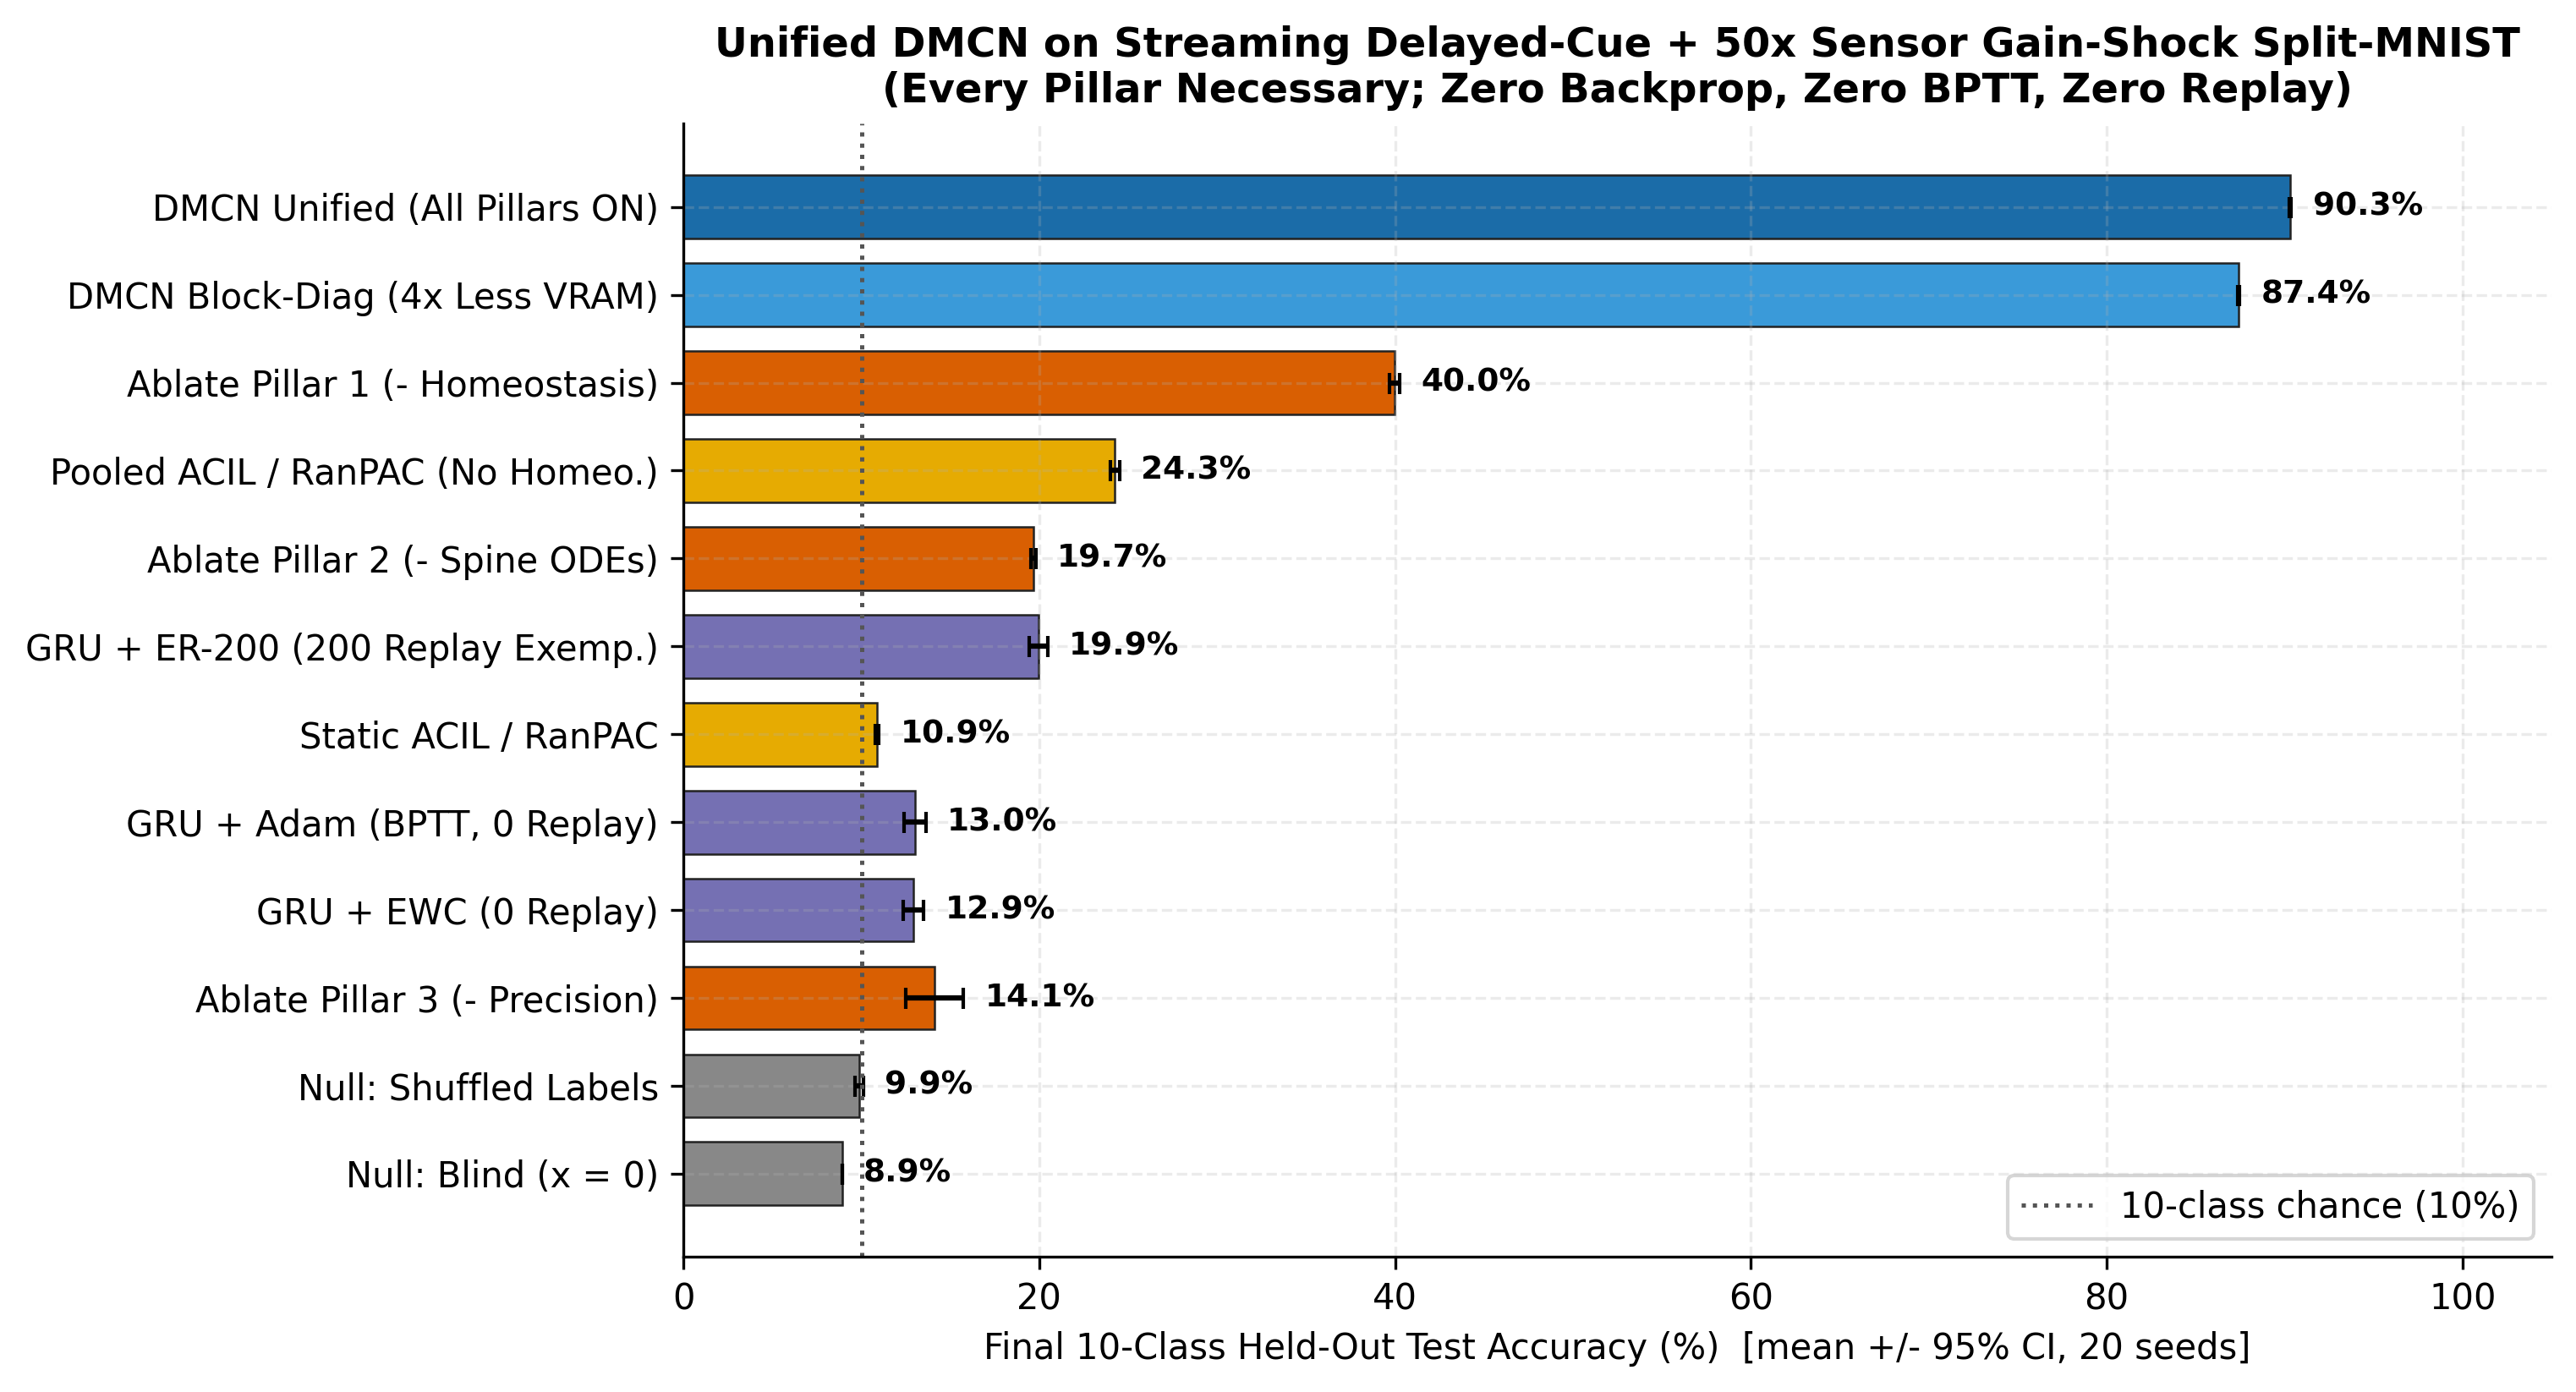
\includegraphics[width=0.96\linewidth]{fig1_unified_all_pillars_ablation.png}
    \caption{Streaming delayed-cue + $50\times$ gain-shock \texttt{Split-MNIST} ($n=20$, $0$ replay). Intact DMCN ($90.32\% \pm 0.06\%$) and 4-branch block-diagonal DMCN ($87.42\%$, $3.99\times$ less VRAM) vs.\ ablations, ACIL, GRUs, and null controls.}
    \label{fig:unified}
\end{figure}

\begin{figure}[htbp]
    \centering
    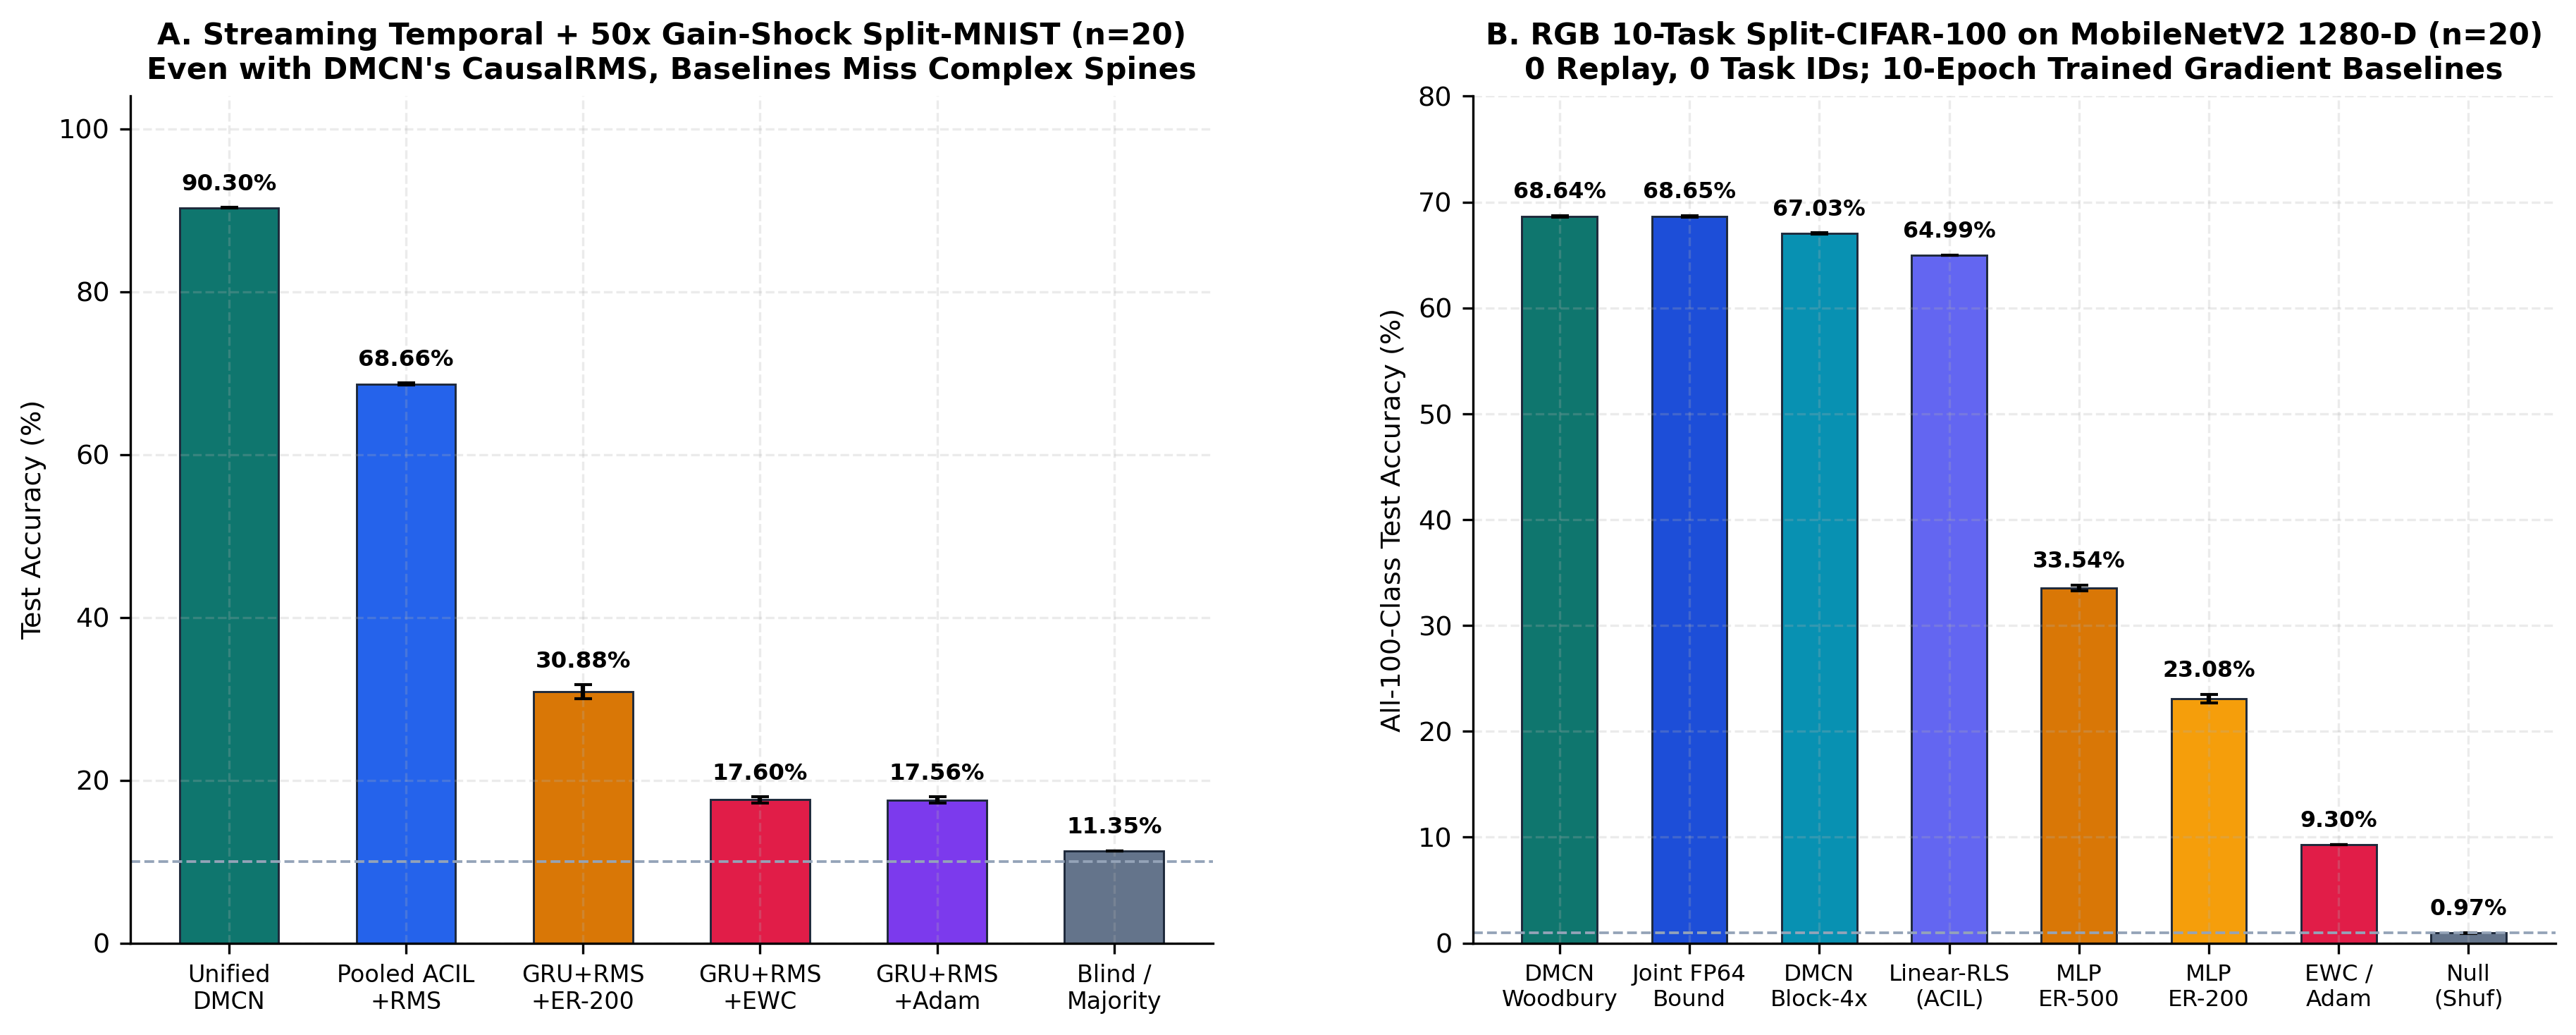
\includegraphics[width=0.98\linewidth]{fig12_reviewer_controls.png}
    \caption{Fairness controls ($n=20$). \textbf{(A)} Even when rival models receive DMCN's \texttt{CausalRMS} normalizer, DMCN leads \texttt{Pooled ACIL + CausalRMS} by $+21.64\text{ pp}$ via complex spine phase memory. \textbf{(B)} On 10-task RGB \texttt{Split-CIFAR-100} (\texttt{MobileNetV2} features), single-pass DMCN matches offline FP64 ridge within $0.0035\%$ and doubles 10-epoch \texttt{ER-500}.}
    \label{fig:controls}
\end{figure}

\begin{table}[htbp]
\centering
\caption{Streaming Delayed-Cue + $50\times$ Gain-Shock \texttt{Split-MNIST} ($n=20$ seeds, 1 pass, $0$ Task IDs).}
\label{tab:temporal}
\small
\resizebox{\linewidth}{!}{%
\begin{tabular}{@{}lrrrr@{}}
\toprule
\textbf{Model / Ablation / Baseline} & \textbf{10-Class Acc ($\text{mean} \pm 95\%\text{ CI}$)} & \textbf{SD} & \textbf{Min--Max} & \textbf{Replay} \\
\midrule
\textbf{DMCN Unified (All Pillars ON)} & \textbf{$90.32\% \pm 0.06\%$} (P0 ret: $97.77\%$) & $0.14\%$ & $90.02\text{--}90.54\%$ & \textbf{0} \\
\textbf{DMCN Block-Diag (4 blocks, $3.99\times$ less VRAM)} & \textbf{$87.42\% \pm 0.06\%$} & $0.13\%$ & $87.15\text{--}87.68\%$ & \textbf{0} \\
Ablate Pillar 1 ($-$ Homeostasis) & $39.96\% \pm 0.29\%$ & $0.66\%$ & $38.95\text{--}41.01\%$ & 0 \\
Ablate Pillar 2 ($-$ Spine ODEs) & $19.66\% \pm 0.14\%$ & $0.31\%$ & $19.03\text{--}20.28\%$ & 0 \\
Ablate Pillar 3 ($-$ Precision Matrix) & $14.11\% \pm 1.62\%$ & $3.70\%$ & $10.09\text{--}18.75\%$ & 0 \\
Pooled ACIL / Static ACIL (raw) & $24.26\%$ / $10.88\%$ & $0.24\text{--}0.56\%$ & $10.56\text{--}25.05\%$ & 0 \\
PyTorch GRU + \texttt{ER-200} / \texttt{Adam} / \texttt{EWC} (raw) & $19.94\%$ / $13.01\%$ / $12.92\%$ & $1.21\text{--}1.39\%$ & $10.31\text{--}22.13\%$ & 200 / 0 / 0 \\
\textit{Fairness Control:} Unified DMCN & \textbf{$90.30\% \pm 0.06\%$} (P0 ret: $97.78\%$) & $0.13\%$ & $90.09\text{--}90.49\%$ & \textbf{0} \\
\textit{Fairness Control:} \texttt{Pooled ACIL + CausalRMS} & $68.66\% \pm 0.11\%$ & $0.24\%$ & $68.25\text{--}69.19\%$ & 0 \\
\textit{Fairness Control:} \texttt{GRU + CausalRMS + ER-200} & $30.88\% \pm 0.85\%$ (P0 ret: $42.58\%$) & $1.94\%$ & $26.68\text{--}34.12\%$ & 200 \\
\textit{Fairness Control:} \texttt{GRU + CausalRMS} (\texttt{EWC}/\texttt{Adam}) & $17.60\%$ / $17.56\%$ & $0.85\text{--}0.86\%$ & $15.59\text{--}18.94\%$ & 0 \\
Nulls (Untrained / Blind / Shuffled / Majority) & $9.80\%$ / $8.92\%$ / $9.88\%$ / $11.35\%$ & $0.00\text{--}0.49\%$ & $8.92\text{--}11.35\%$ & --- \\
\bottomrule
\end{tabular}}
\end{table}

\subsection{RGB \texttt{Split-CIFAR-100}, Static Continual Baselines, GPU Speed, and \texorpdfstring{$95\%$}{95\%} Sparsity}
On 10-task RGB \texttt{Split-CIFAR-100} (frozen ImageNet \texttt{MobileNetV2} $1280\text{-D} \to 5{,}377\text{-D}$ features, $0$ replay, $0$ task IDs) as well as static \texttt{Split-MNIST} and \texttt{Split-FashionMNIST}, DMCN matches the offline joint FP64 ridge upper bound within $0.0005\text{--}0.0040\text{ pp}$ in a single pass (Figure~\ref{fig:controls}B, Figure~\ref{fig:cl_lit}, Table~\ref{tab:cl_all}). Replacing per-batch Woodbury solves with checkpointed \textbf{Gram--Cholesky} accelerates RTX 3060 GPU training $3.86\times$ on \texttt{Split-MNIST} ($81{,}936$ samples/s vs.\ $21{,}224$, and $82{,}467$ samples/s / $3.89\times$ with ternary weights, compared to Backprop Adam's $120{,}716$/s) and $2.62\times$ on \texttt{Split-CIFAR-100} ($2.58\text{ s}$ vs.\ $6.76\text{ s}$), while $95\%$ sparse ternary $\{-1,0,+1\}$ L1 projections retain exact $68.65\%$ CIFAR-100 accuracy with $20\times$ fewer nonzero Layer-1 weights (Figure~\ref{fig:v4}A--B, Table~\ref{tab:gpu}).

\begin{figure}[htbp]
    \centering
    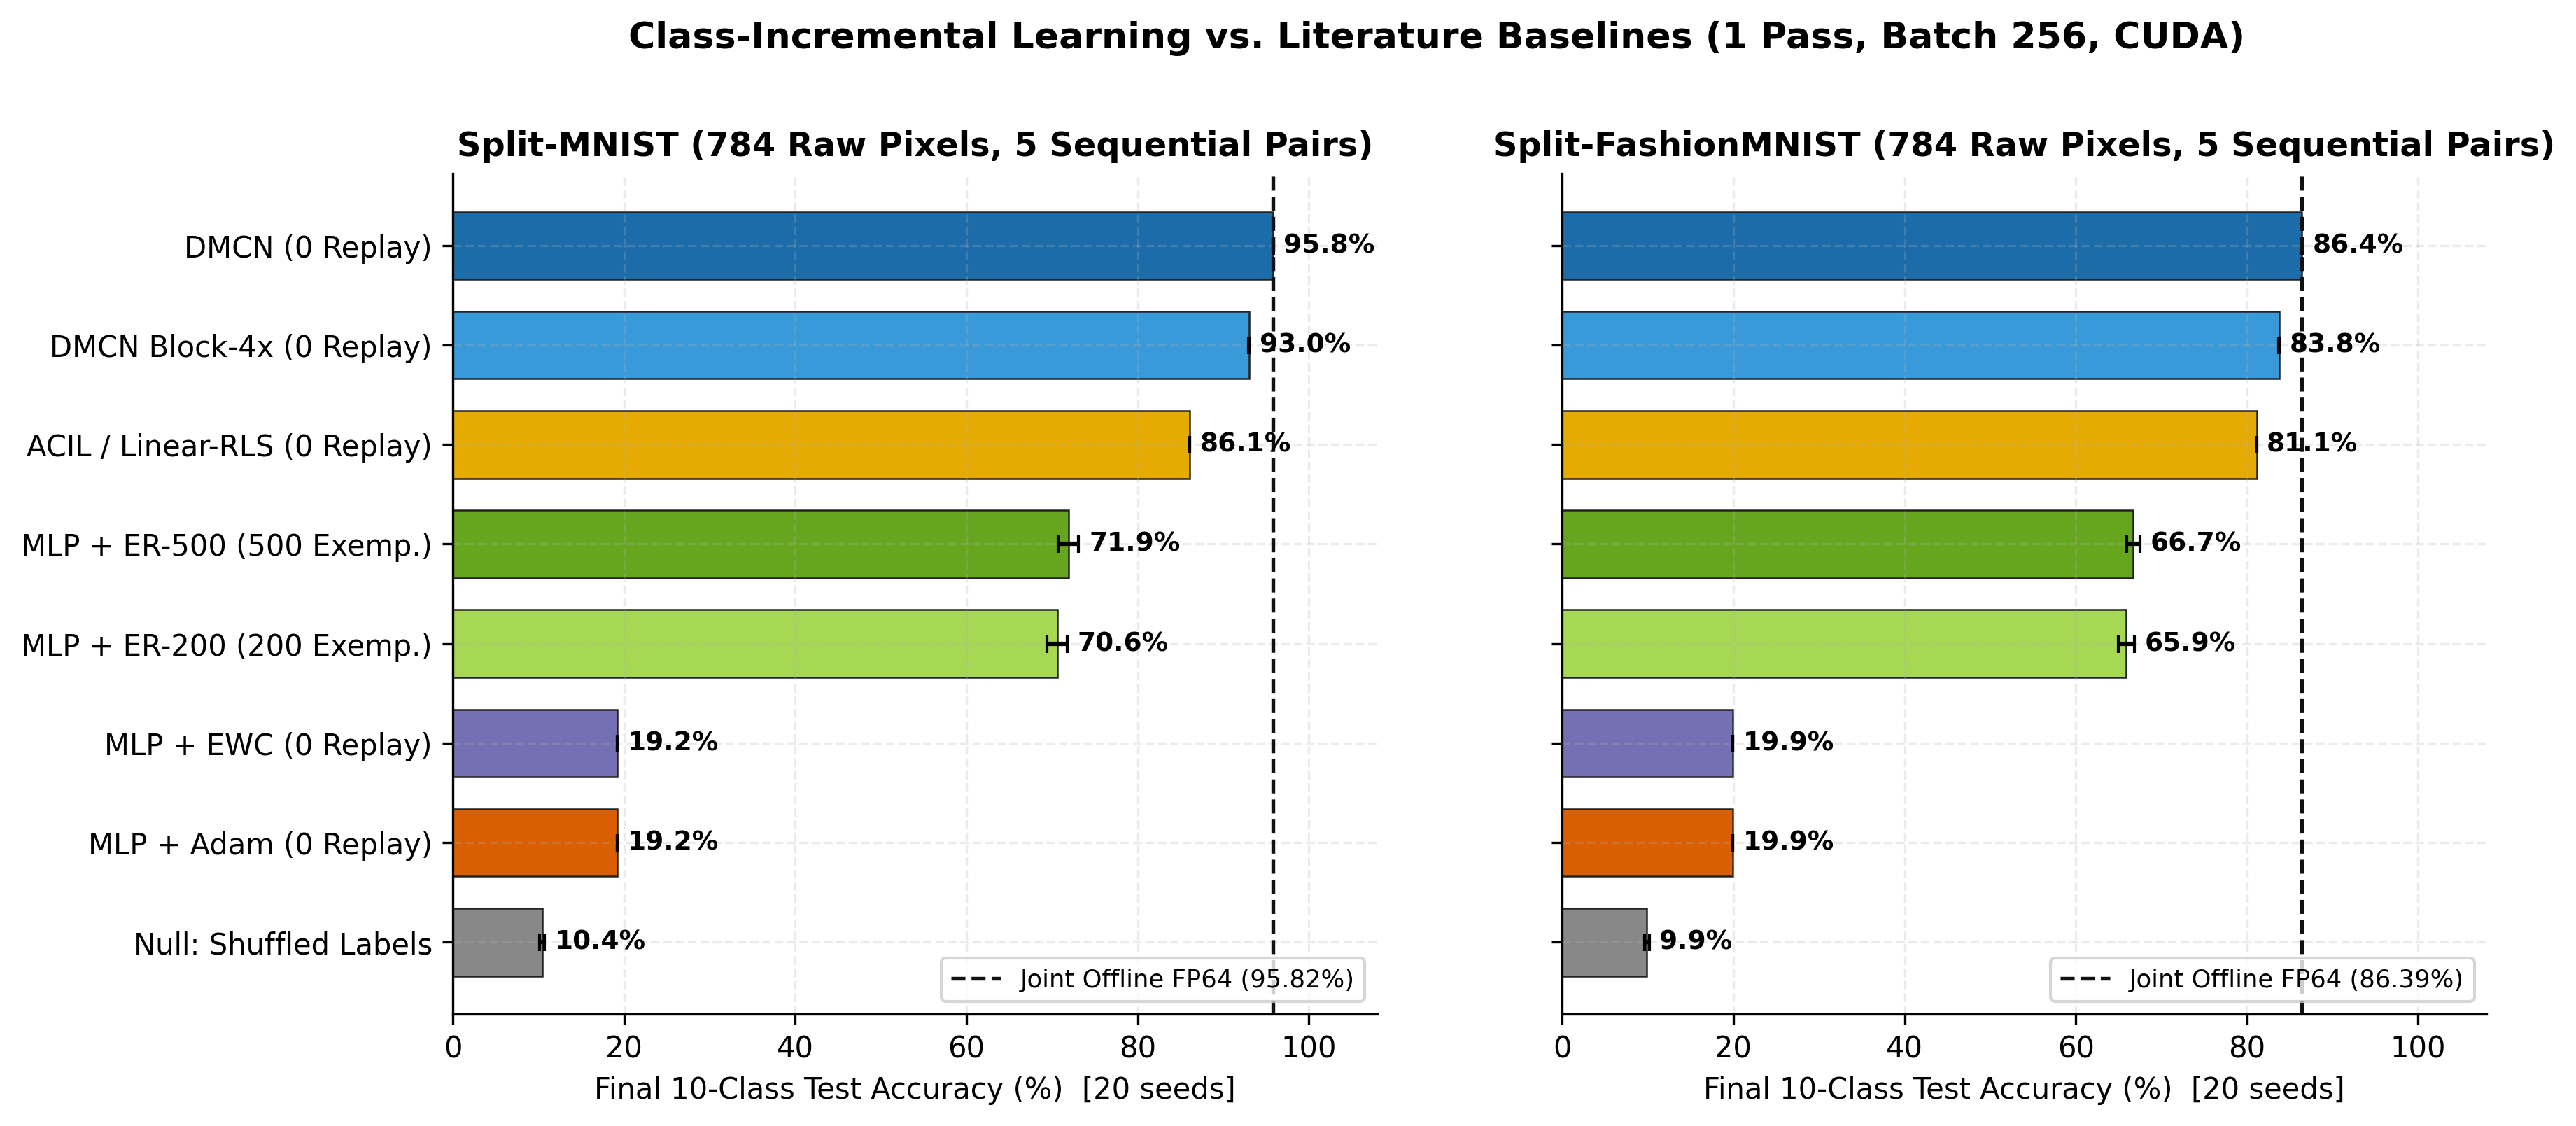
\includegraphics[width=0.98\linewidth]{fig2_cl_literature_baselines.png}
    \caption{Static 1-pass \texttt{Split-MNIST} and \texttt{Split-FashionMNIST} ($n=20$, $0$ replay) vs.\ \texttt{ACIL/Linear-RLS}, \texttt{ER-200/500}, \texttt{EWC}, \texttt{Adam}, and joint offline FP64 ridge bounds.}
    \label{fig:cl_lit}
\end{figure}

\begin{figure}[htbp]
    \centering
    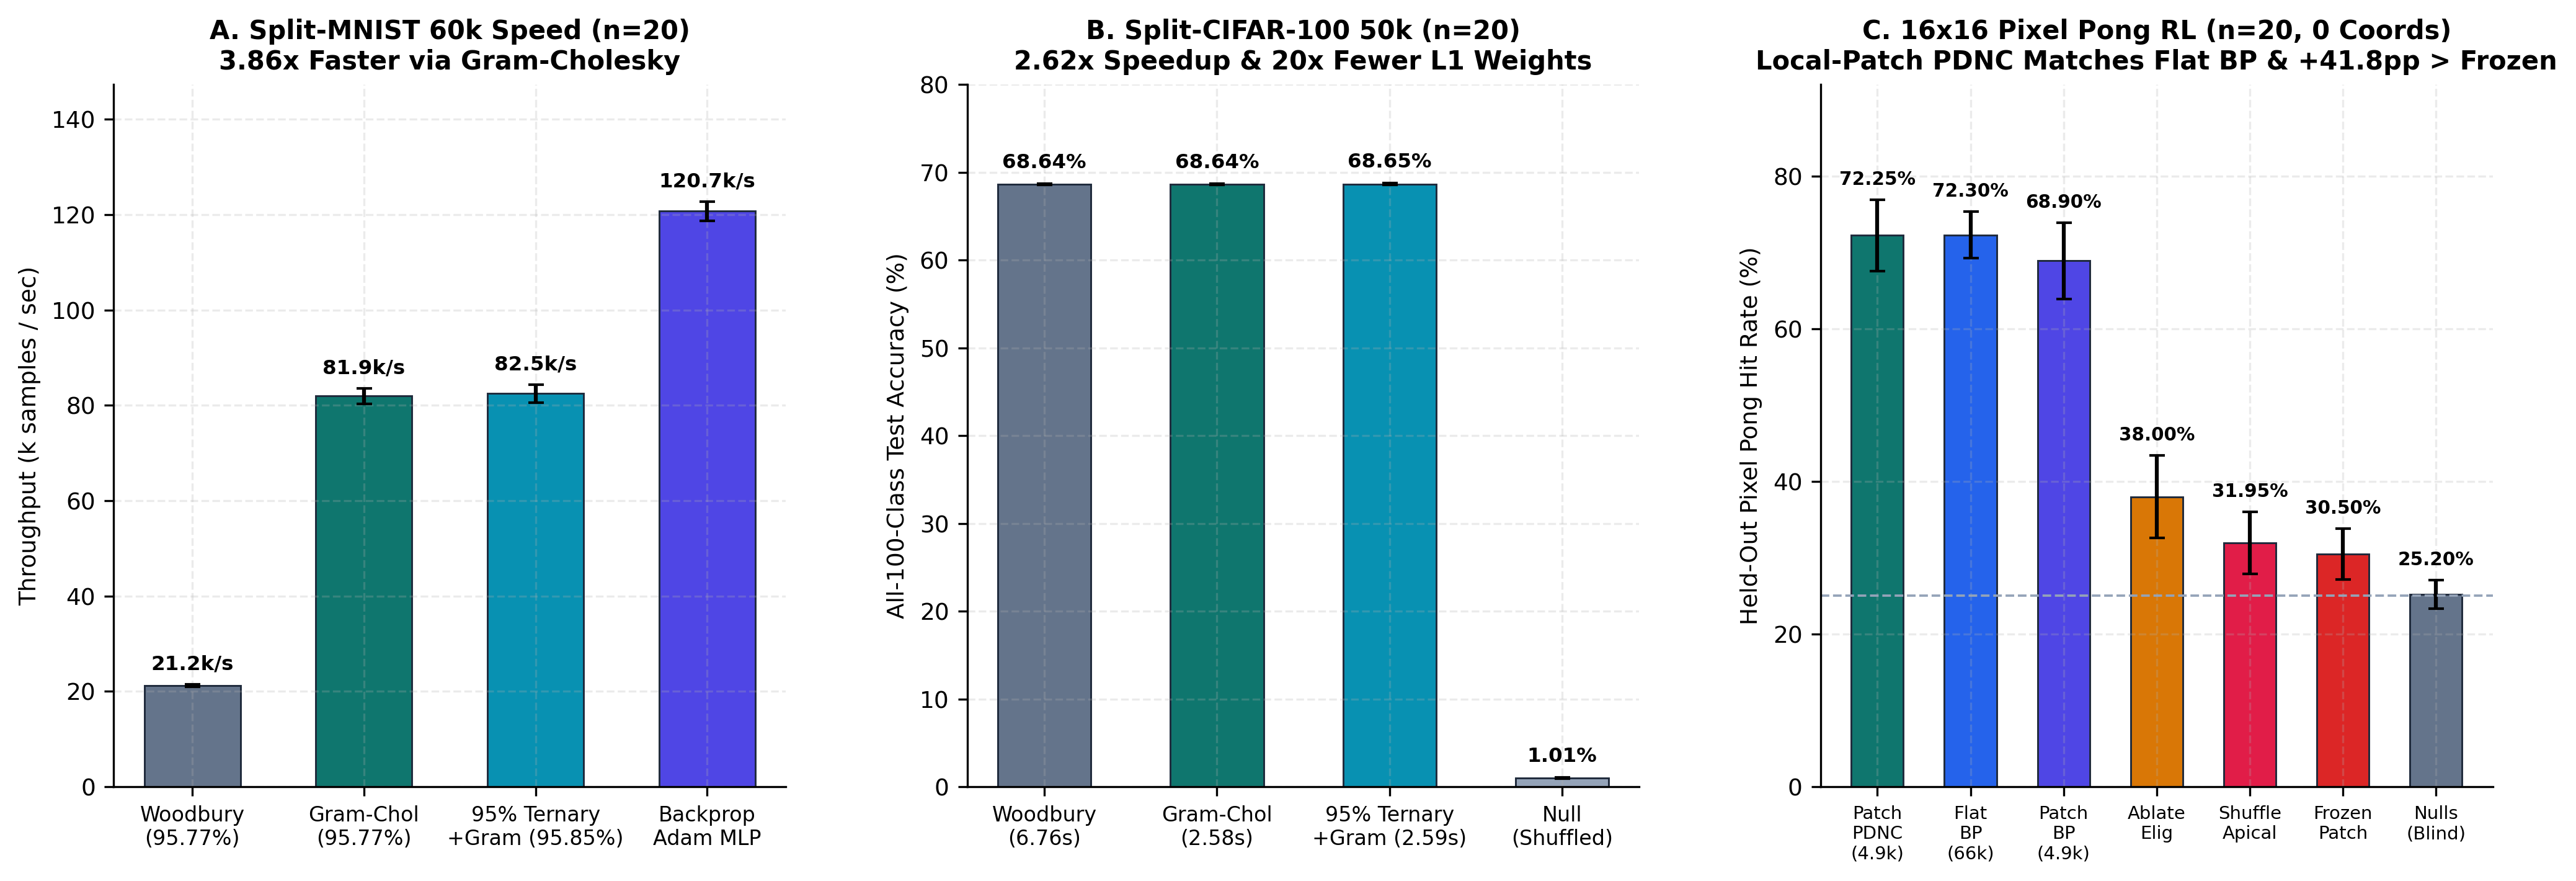
\includegraphics[width=0.98\linewidth]{fig13_dmcn_v4_efficiency_and_patch_pdnc.png}
    \caption{GPU speed, ternary sparsity, and local-patch RL ($n=20$). \textbf{(A)} Gram--Cholesky gives $3.86\times$ \texttt{Split-MNIST} speedup ($81.9\text{k}/s$). \textbf{(B)} $95\%$ sparse ternary + Gram preserves $68.65\%$ CIFAR-100 in $2.59\text{ s}$. \textbf{(C)} Overlapping $4\times 4$ \texttt{Local-Patch PDNC} hits $72.25\%$ on raw Pixel Pong, tying Flat Backprop A2C ($72.30\%$) with $13.5\times$ fewer L1 synapses.}
    \label{fig:v4}
\end{figure}

\begin{table}[htbp]
\centering
\caption{Continual Learning on RGB \texttt{Split-CIFAR-100}, \texttt{Split-MNIST}, and \texttt{Split-FashionMNIST} ($n=20$).}
\label{tab:cl_all}
\small
\resizebox{\linewidth}{!}{%
\begin{tabular}{@{}lrrrrr@{}}
\toprule
\textbf{Method} & \textbf{Ep/Task} & \textbf{Replay} & \textbf{Split-CIFAR-100 (\%)} & \textbf{Split-MNIST (\%)} & \textbf{Split-FMNIST (\%)} \\
\midrule
\textbf{DMCN (Woodbury, 0 BP)} & \textbf{1} & \textbf{0} & \textbf{$68.65 \pm 0.09$} (T0: $70.60\%$) & \textbf{$95.82 \pm 0.05$} (P0: $98.83\%$) & \textbf{$86.39 \pm 0.05$} (P0: $89.41\%$) \\
Joint Offline FP64 Bound & Offline & All & $68.65 \pm 0.09$ (gap $0.0035\%$) & $95.82 \pm 0.05$ (gap $0.0005\%$) & $86.39 \pm 0.05$ (gap $0.0040\%$) \\
\textbf{DMCN Block-Diag (4 blocks)} & \textbf{1} & \textbf{0} & \textbf{$67.03 \pm 0.05$} & \textbf{$93.01 \pm 0.05$} & \textbf{$83.75 \pm 0.04$} \\
\texttt{Linear-RLS / ACIL} & 1 & 0 & $64.99 \pm 0.00$ (val-tuned) & $86.09 \pm 0.00$ & $81.12 \pm 0.00$ \\
\texttt{MLP + ER-500} ($10$ ep C100) & 10 / 1 & 500 & $33.54 \pm 0.27$ & $71.92 \pm 1.20$ & $66.71 \pm 0.78$ \\
\texttt{MLP + ER-200} ($10$ ep C100) & 10 / 1 & 200 & $23.08 \pm 0.40$ & $70.61 \pm 1.17$ & $65.89 \pm 0.95$ \\
\texttt{MLP + EWC} / \texttt{Adam} & 10 / 1 & 0 & $9.30$ / $9.31$ & $19.22$ / $19.22$ & $19.93$ / $19.93$ \\
Nulls (Untr / Blind / Shuf / Maj) & --- & 0 & $1.00/1.00/0.97/1.00$ & $9.80/9.80/10.43/11.35$ & $10.00/10.00/9.89/10.00$ \\
\bottomrule
\end{tabular}}
\end{table}

\begin{table}[htbp]
\centering
\caption{GPU Throughput, Algebraic Parity, and $95\%$ Sparse Ternary Ablation ($n=20$, RTX 3060).}
\label{tab:gpu}
\small
\resizebox{\linewidth}{!}{%
\begin{tabular}{@{}lrrrr@{}}
\toprule
\textbf{Variant ($n=20$)} & \textbf{MNIST Acc (\%)} & \textbf{MNIST Speed (samp/s)} & \textbf{C100 Acc (\%)} & \textbf{C100 Time (s) / VRAM} \\
\midrule
Woodbury ($P$ per mini-batch) & $95.77 \pm 0.05$ & $21{,}224 \pm 296$ & $68.64 \pm 0.07$ & $6.76 \pm 0.07$ ($1{,}432.7\text{ MB}$) \\
\textbf{Gram--Cholesky} & \textbf{$95.77 \pm 0.05$} & \textbf{$81{,}936 \pm 1{,}593$ ($3.86\times$)} & \textbf{$68.64 \pm 0.07$} & \textbf{$2.58 \pm 0.03$ ($2.62\times$)} ($1{,}409.9\text{ MB}$) \\
\textbf{95\% Ternary + Gram} & \textbf{$95.85 \pm 0.04$} & \textbf{$82{,}467 \pm 1{,}898$ ($3.89\times$)} & \textbf{$68.65 \pm 0.10$} & \textbf{$2.59 \pm 0.03$} ($20\times$ fewer L1 nz) \\
Backprop Adam MLP (ref) & \textit{(forgets old)} & $120{,}716 \pm 2{,}043$ & \textit{(forgets old)} & --- \\
Null: Shuffled Labels & --- & --- & $1.01 \pm 0.05$ & --- \\
\bottomrule
\end{tabular}}
\end{table}

\subsection{Autonomous Pathway Gating and Zero-Shot Compositionality}
Under one frozen self-gating configuration ($n=20$, zero task IDs), Hedge gating routes $85.26\%$ weight to \texttt{raw+transient} on Lorenz chaos ($0.0054 \pm 0.0013$ NMSE), reallocates $90.39\%$ to \texttt{homeo+spine} under $100\times$ $[0.2, 20.0]$ gain shocks ($0.0928 \pm 0.0103$ vs.\ $0.2021$ raw-only), and achieves $100.00\%$ on 4-step delayed cues ($45.42\%$ spine, $0.003\%$ raw; Figure~\ref{fig:selfgate}). Under column permutations, competitive sparse Oja factorization + bilinear coincidence reaches \textbf{$98.05\% \pm 2.27\%$} on unseen \texttt{Color $\times$ Shape} and \textbf{$99.58\% \pm 0.82\%$} ($\text{MSE } 0.0017$) on unseen \texttt{Rule $\times$ Operand}, beating Backprop Adam ($83.75\%$), whereas ablating bilinear products drops to $10.83\%$ (Figure~\ref{fig:comp}, Table~\ref{tab:gate_comp}).

\begin{figure}[htbp]
    \centering
    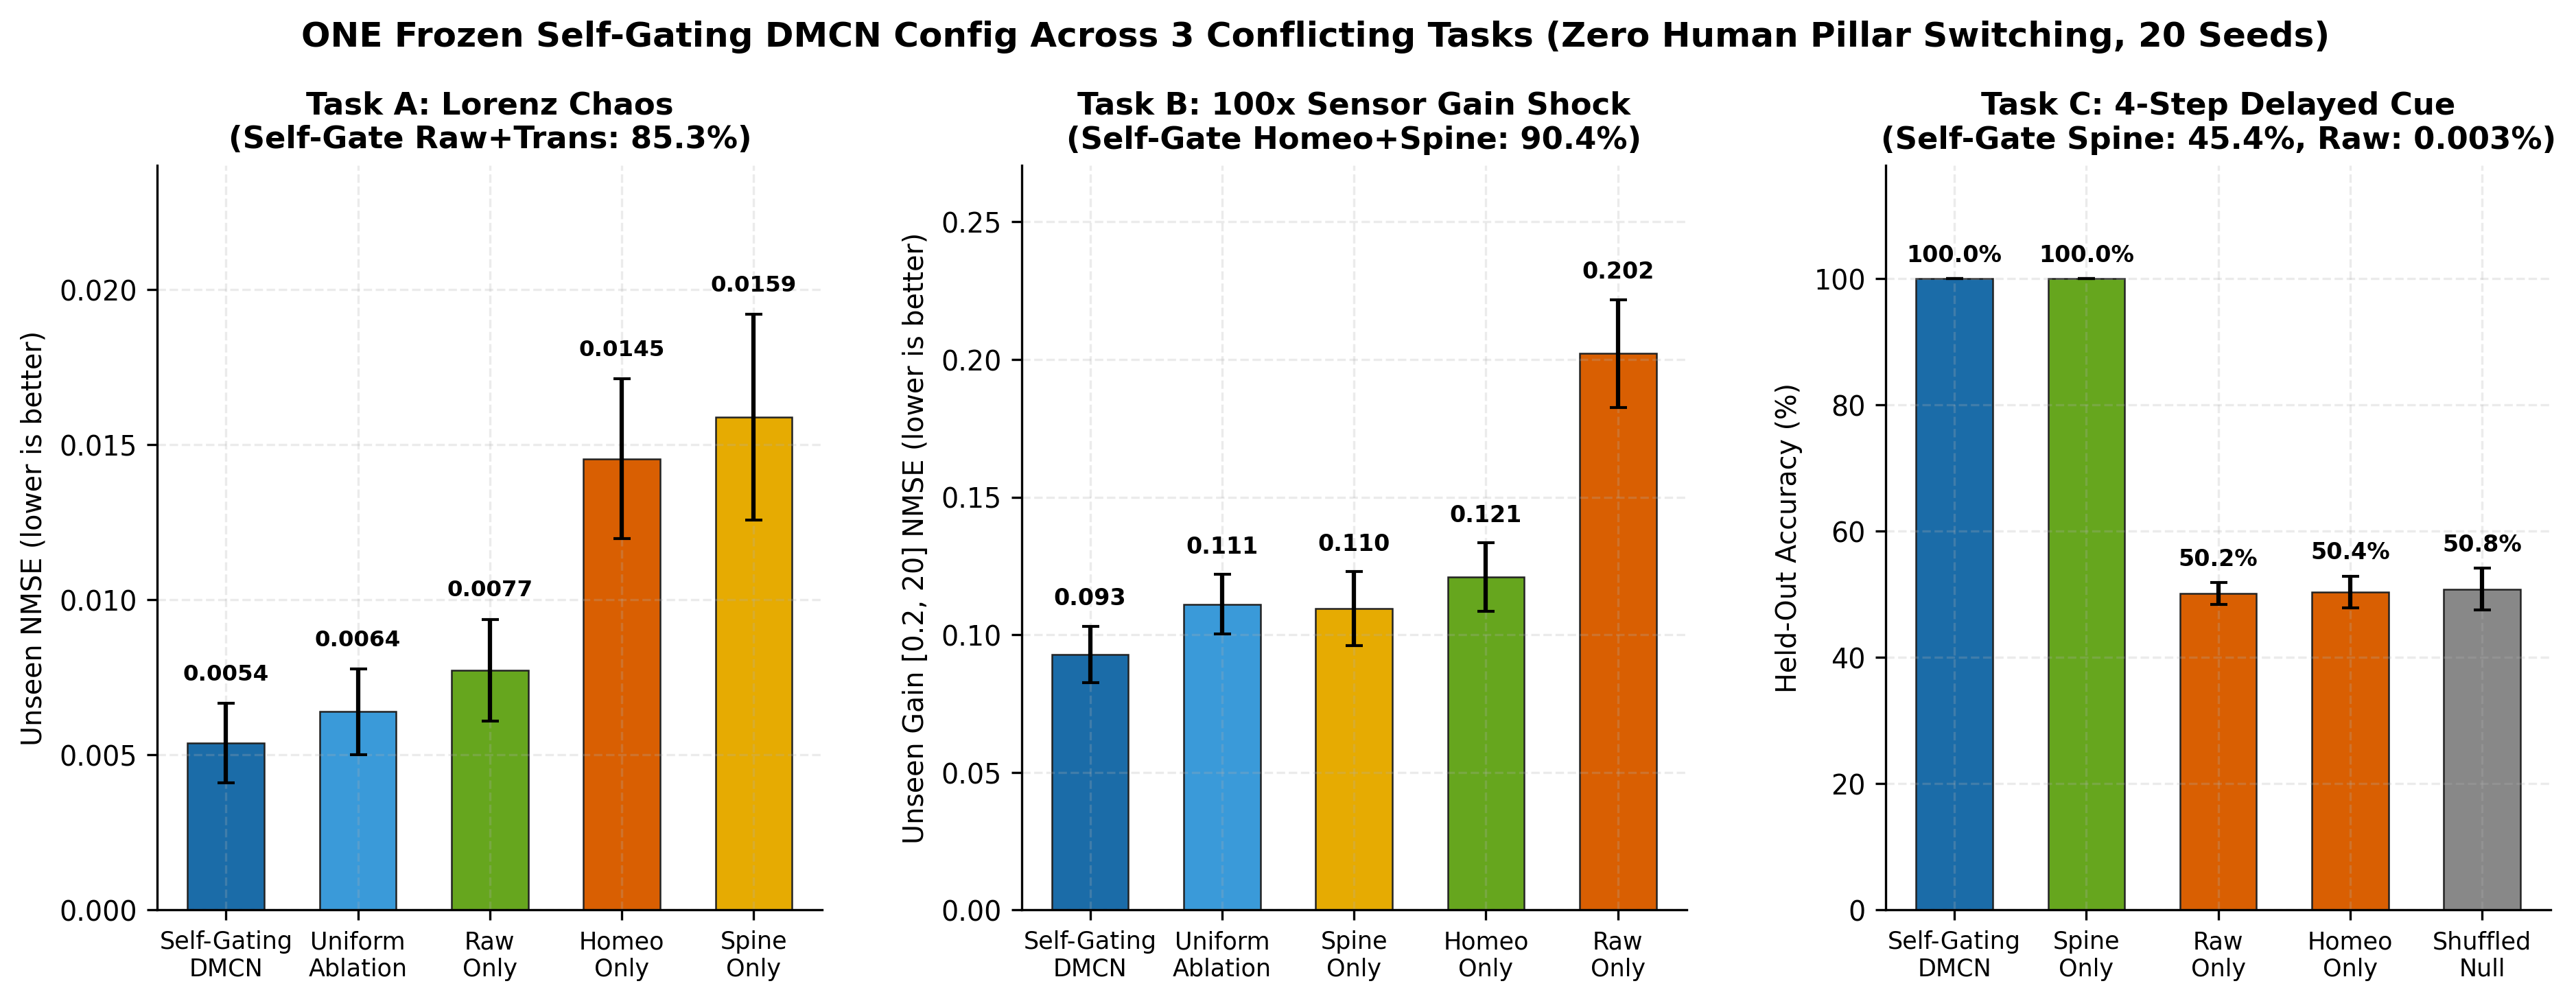
\includegraphics[width=0.98\linewidth]{fig8_self_gating_unified.png}
    \caption{One frozen self-gating DMCN configuration adapts weights automatically across Lorenz chaos ($85.3\%$ \texttt{raw+trans}), $100\times$ gain shocks ($90.4\%$ \texttt{homeo+spine}), and 4-step delayed cues ($n=20$).}
    \label{fig:selfgate}
\end{figure}

\begin{figure}[htbp]
    \centering
    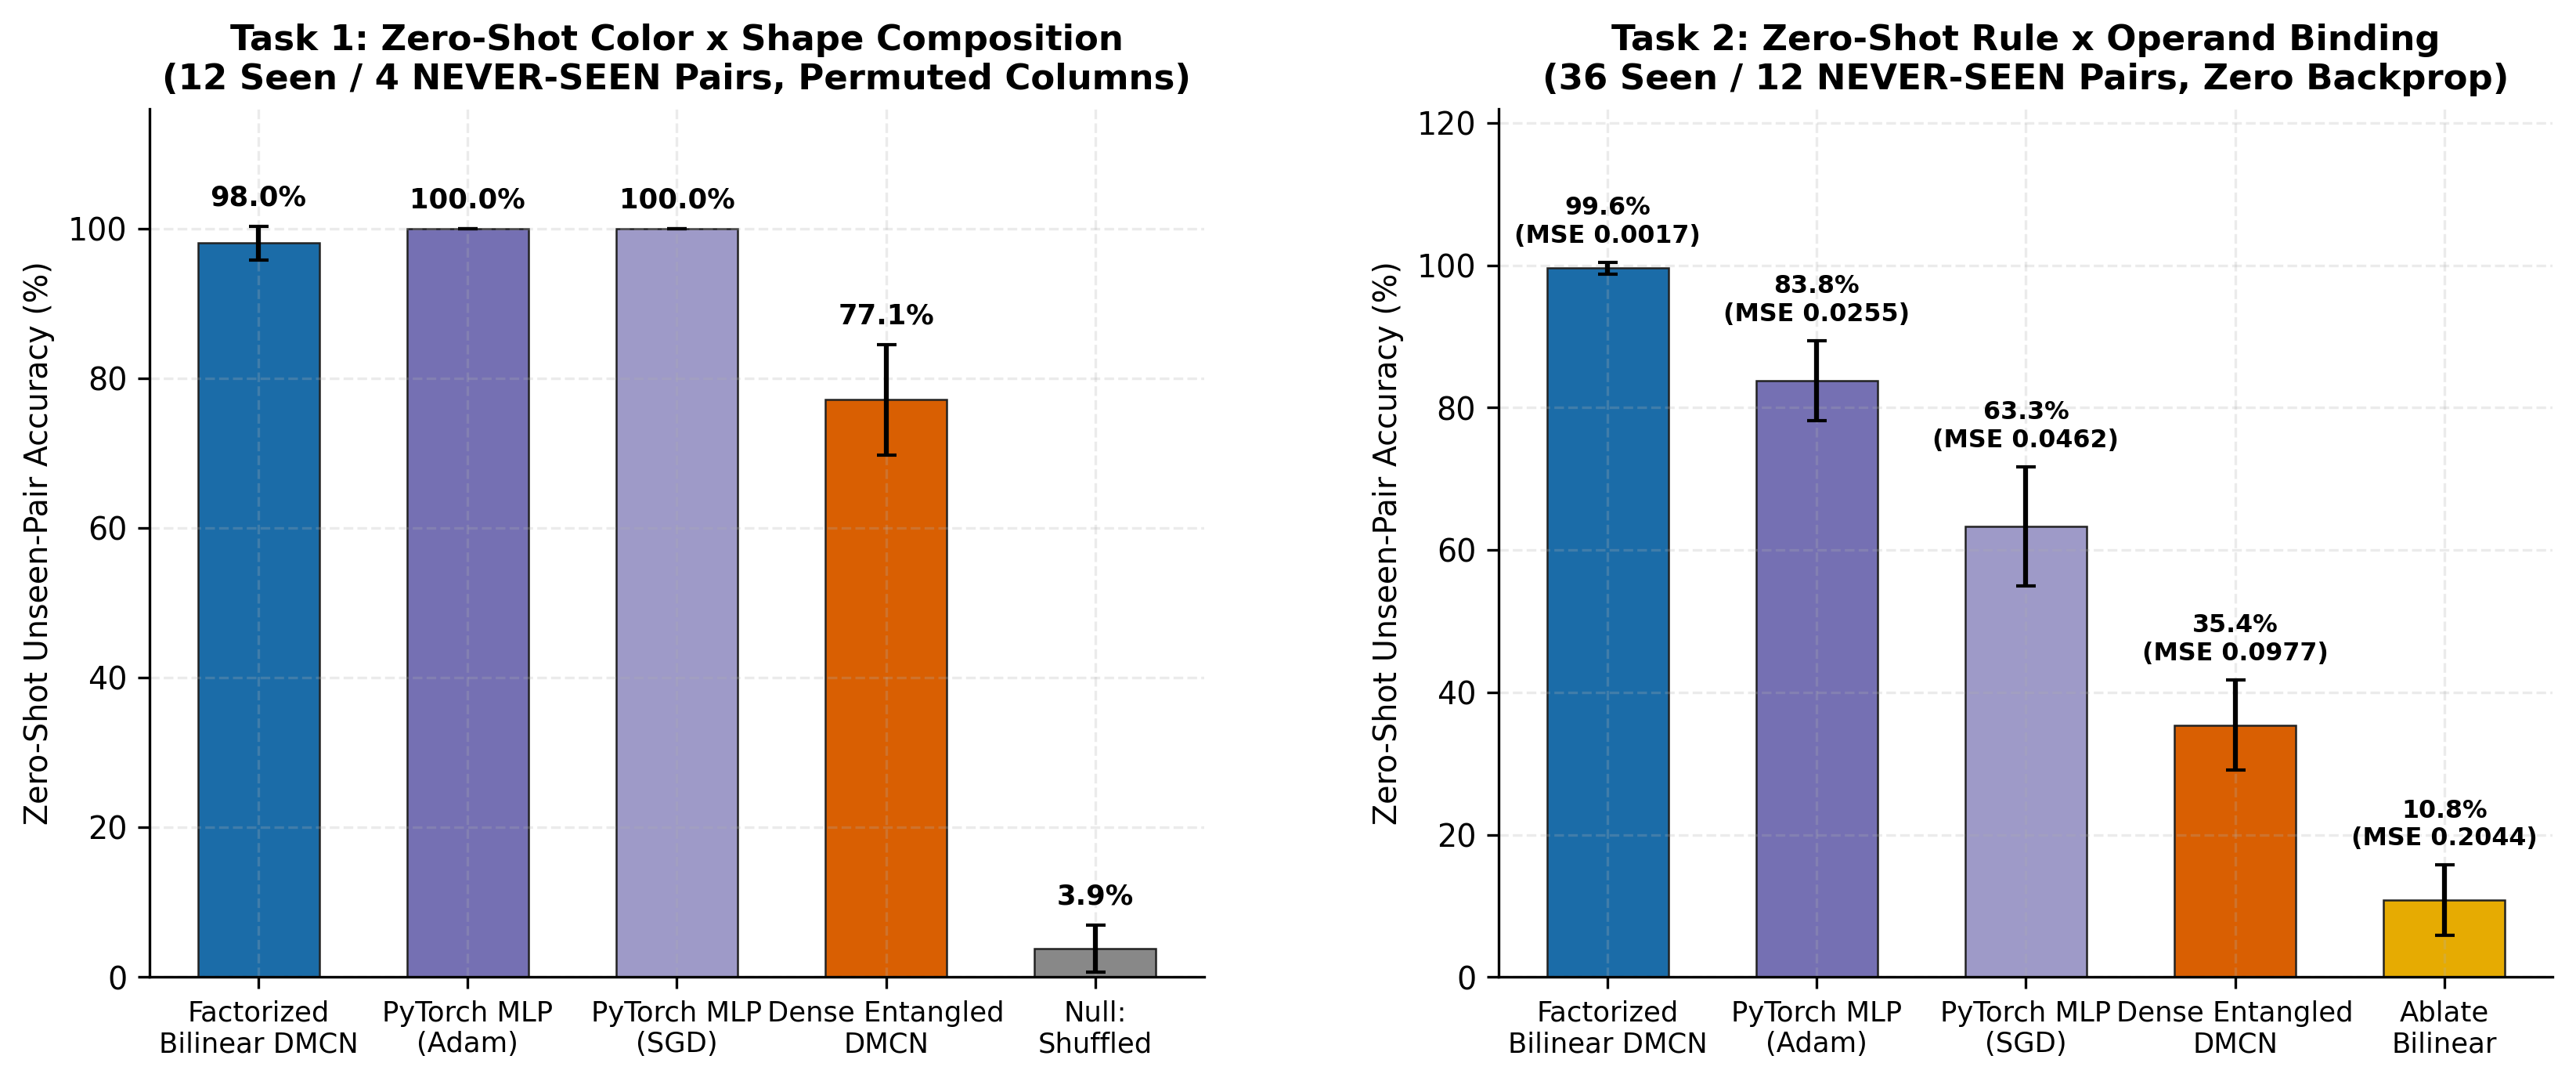
\includegraphics[width=0.98\linewidth]{fig9_compositional_generalization.png}
    \caption{Zero-shot generalization with permuted columns ($n=20$): competitive Oja factorization + bilinear coincidence reaches $98.05\%$ on unseen \texttt{Color $\times$ Shape} and $99.58\%$ ($\text{MSE } 0.0017$) on unseen \texttt{Rule $\times$ Operand}.}
    \label{fig:comp}
\end{figure}

\begin{table}[htbp]
\centering
\caption{Autonomous Self-Gating ($n=20$) and Zero-Shot Compositional Binding ($n=20$).}
\label{tab:gate_comp}
\small
\resizebox{\linewidth}{!}{%
\begin{tabular}{@{}lllll@{}}
\toprule
\textbf{Task} & \textbf{Primary DMCN} & \textbf{Ablation / Uniform} & \textbf{Backprop Ref} & \textbf{Null Control} \\
\midrule
Lorenz Chaos NMSE ($\downarrow$) & \textbf{$0.0054 \pm 0.0013$} & Uniform $0.0064$, Homeo $0.0146$ & --- & Shuf: $0.3742$ \\
$100\times$ Shock NMSE ($\downarrow$) & \textbf{$0.0928 \pm 0.0103$} & Raw $0.2021$, Uniform $0.1111$ & --- & Shuf: $1.0294$ \\
4-Step Delayed Cue ($\uparrow$) & \textbf{$100.00\% \pm 0.00\%$} & Raw $50.17\%$, Homeo $50.40\%$ & --- & Shuf: $50.83\%$ \\
Unseen \texttt{Color $\times$ Shape} & \textbf{$98.05\% \pm 2.27\%$} & Dense DMCN: $77.10\% \pm 7.40\%$ & Adam/SGD: $100.00\%$ & Shuf/Blind: $3.85/5.00\%$ \\
Unseen \texttt{Rule $\times$ Operand} & \textbf{$99.58\% \pm 0.82\%$} (MSE $0.0017$) & No Bilin: $10.83\%$, Dense: $35.42\%$ & Adam $83.75\%$, SGD $63.33\%$ & Untr/Blind/Shuf: $3.75/1.25/2.08\%$ \\
\bottomrule
\end{tabular}}
\end{table}

\subsection{Local Multi-Layer Visual Learning (\texttt{PDNC}): Unsupervised Failure to Local Patches}
\label{sec:pdnc_results}
On raw $16\times 16$ Pixel Pong ($256$ pixels, $0$ coordinates, sparse $+1/-1$ terminal reward, $2{,}000$ serves), leaving Layer 1 frozen stalled at $47.65\% \pm 3.45\%$ (vs.\ $76.05\%$ intact / $94.35\%$ no-spine on 4-D state vectors). First, unsupervised competitive Motion-Oja on L1 \textbf{refuted} our unsupervised-vision hypothesis (Figure~\ref{fig:oja}): peak pixel energy rose ($0.0898$ vs.\ $0.0640$ frozen), yet hit rate fell from $45.30\% \pm 3.98\%$ to \textbf{$39.05\% \pm 4.02\%$} because unrewarded competition locked onto bright paddles and discarded the tiny ball.

Switching to top-down apical feedback via \textbf{Dense \texttt{PDNC}} (Figure~\ref{fig:pdnc}) lifted raw Pixel Pong to $63.40\% \pm 4.84\%$ ($\text{KP cos} = 0.766$, $+32.85\text{ pp}$ over frozen $30.55\%$), solved 24D Noisy XOR at $84.71\% \pm 1.23\%$ ($12.03\times$ SNR vs.\ $49.84\%$ frozen), and reached $83.28\% \pm 0.81\%$ on boundary-free rotated 3-task CL (beating BP SGD $77.85\%$). However, on compact $d=256$ continual \texttt{Split-FashionMNIST}, plastic L1 weights dropped accuracy below frozen L1 ($70.13\%$ vs.\ $80.72\%$), confirming the hidden-drift interference described in Section~4.

Confining compartments to overlapping \textbf{$4\times 4$ local visual patches} ($147$ compartments, $4{,}851$ L1 synapses---$13.5\times$ fewer than flat $256\to 128$, $0$ weight sharing, $0$ coordinates) pushed \textbf{\texttt{Local-Patch PDNC}} to \textbf{$72.25\% \pm 4.68\%$} ($52.30\%$ OOD, $\text{KP cos} = 0.758$), statistically tying Flat Backprop A2C ($72.30\% \pm 3.05\%$), beating Patch Backprop A2C ($68.90\% \pm 5.01\%$), and gaining $+41.75\text{ pp}$ over Frozen Patch L1 ($30.50\%$; Figure~\ref{fig:v4}C, Table~\ref{tab:pong}). Nevertheless, this missed our pre-registered $74.0\%$ threshold by $1.75\text{ pp}$ and showed higher cross-seed variance ($\text{SD}=10.69\%$, min seed $36.0\%$).

\begin{figure}[htbp]
    \centering
    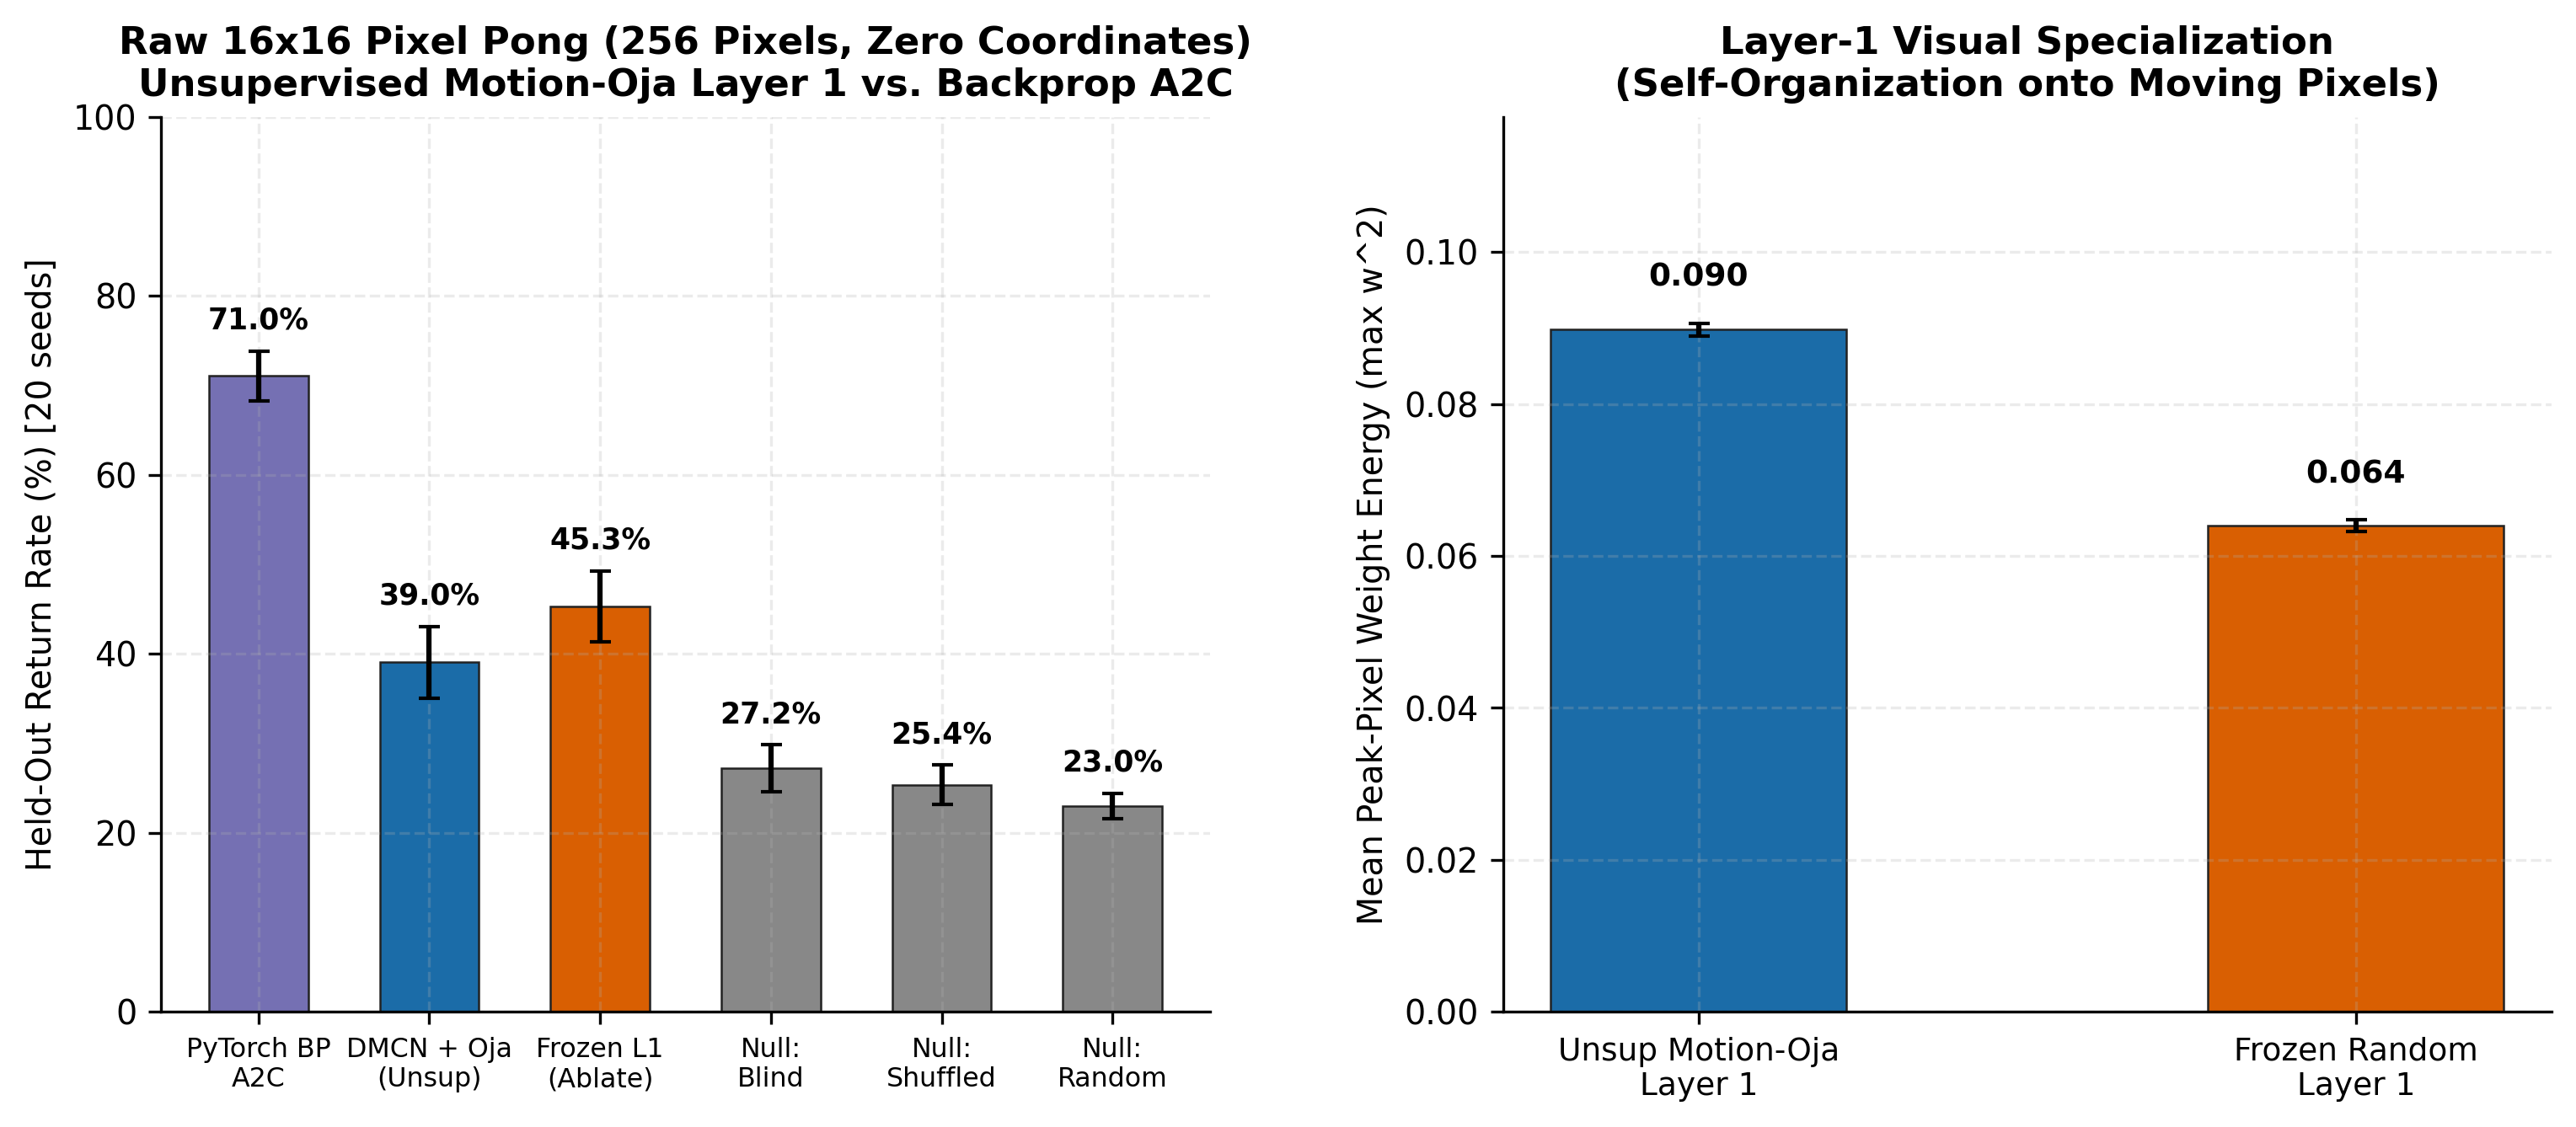
\includegraphics[width=0.96\linewidth]{fig10_pong_pixel_unsup_oja.png}
    \caption{Refuted unsupervised Motion-Oja hypothesis ($n=20$): peak pixel concentration increased ($0.090$ vs.\ $0.064$), but hit rate fell ($39.0\%$ vs.\ $45.3\%$ frozen) due to unrewarded paddle capture.}
    \label{fig:oja}
\end{figure}

\begin{figure}[htbp]
    \centering
    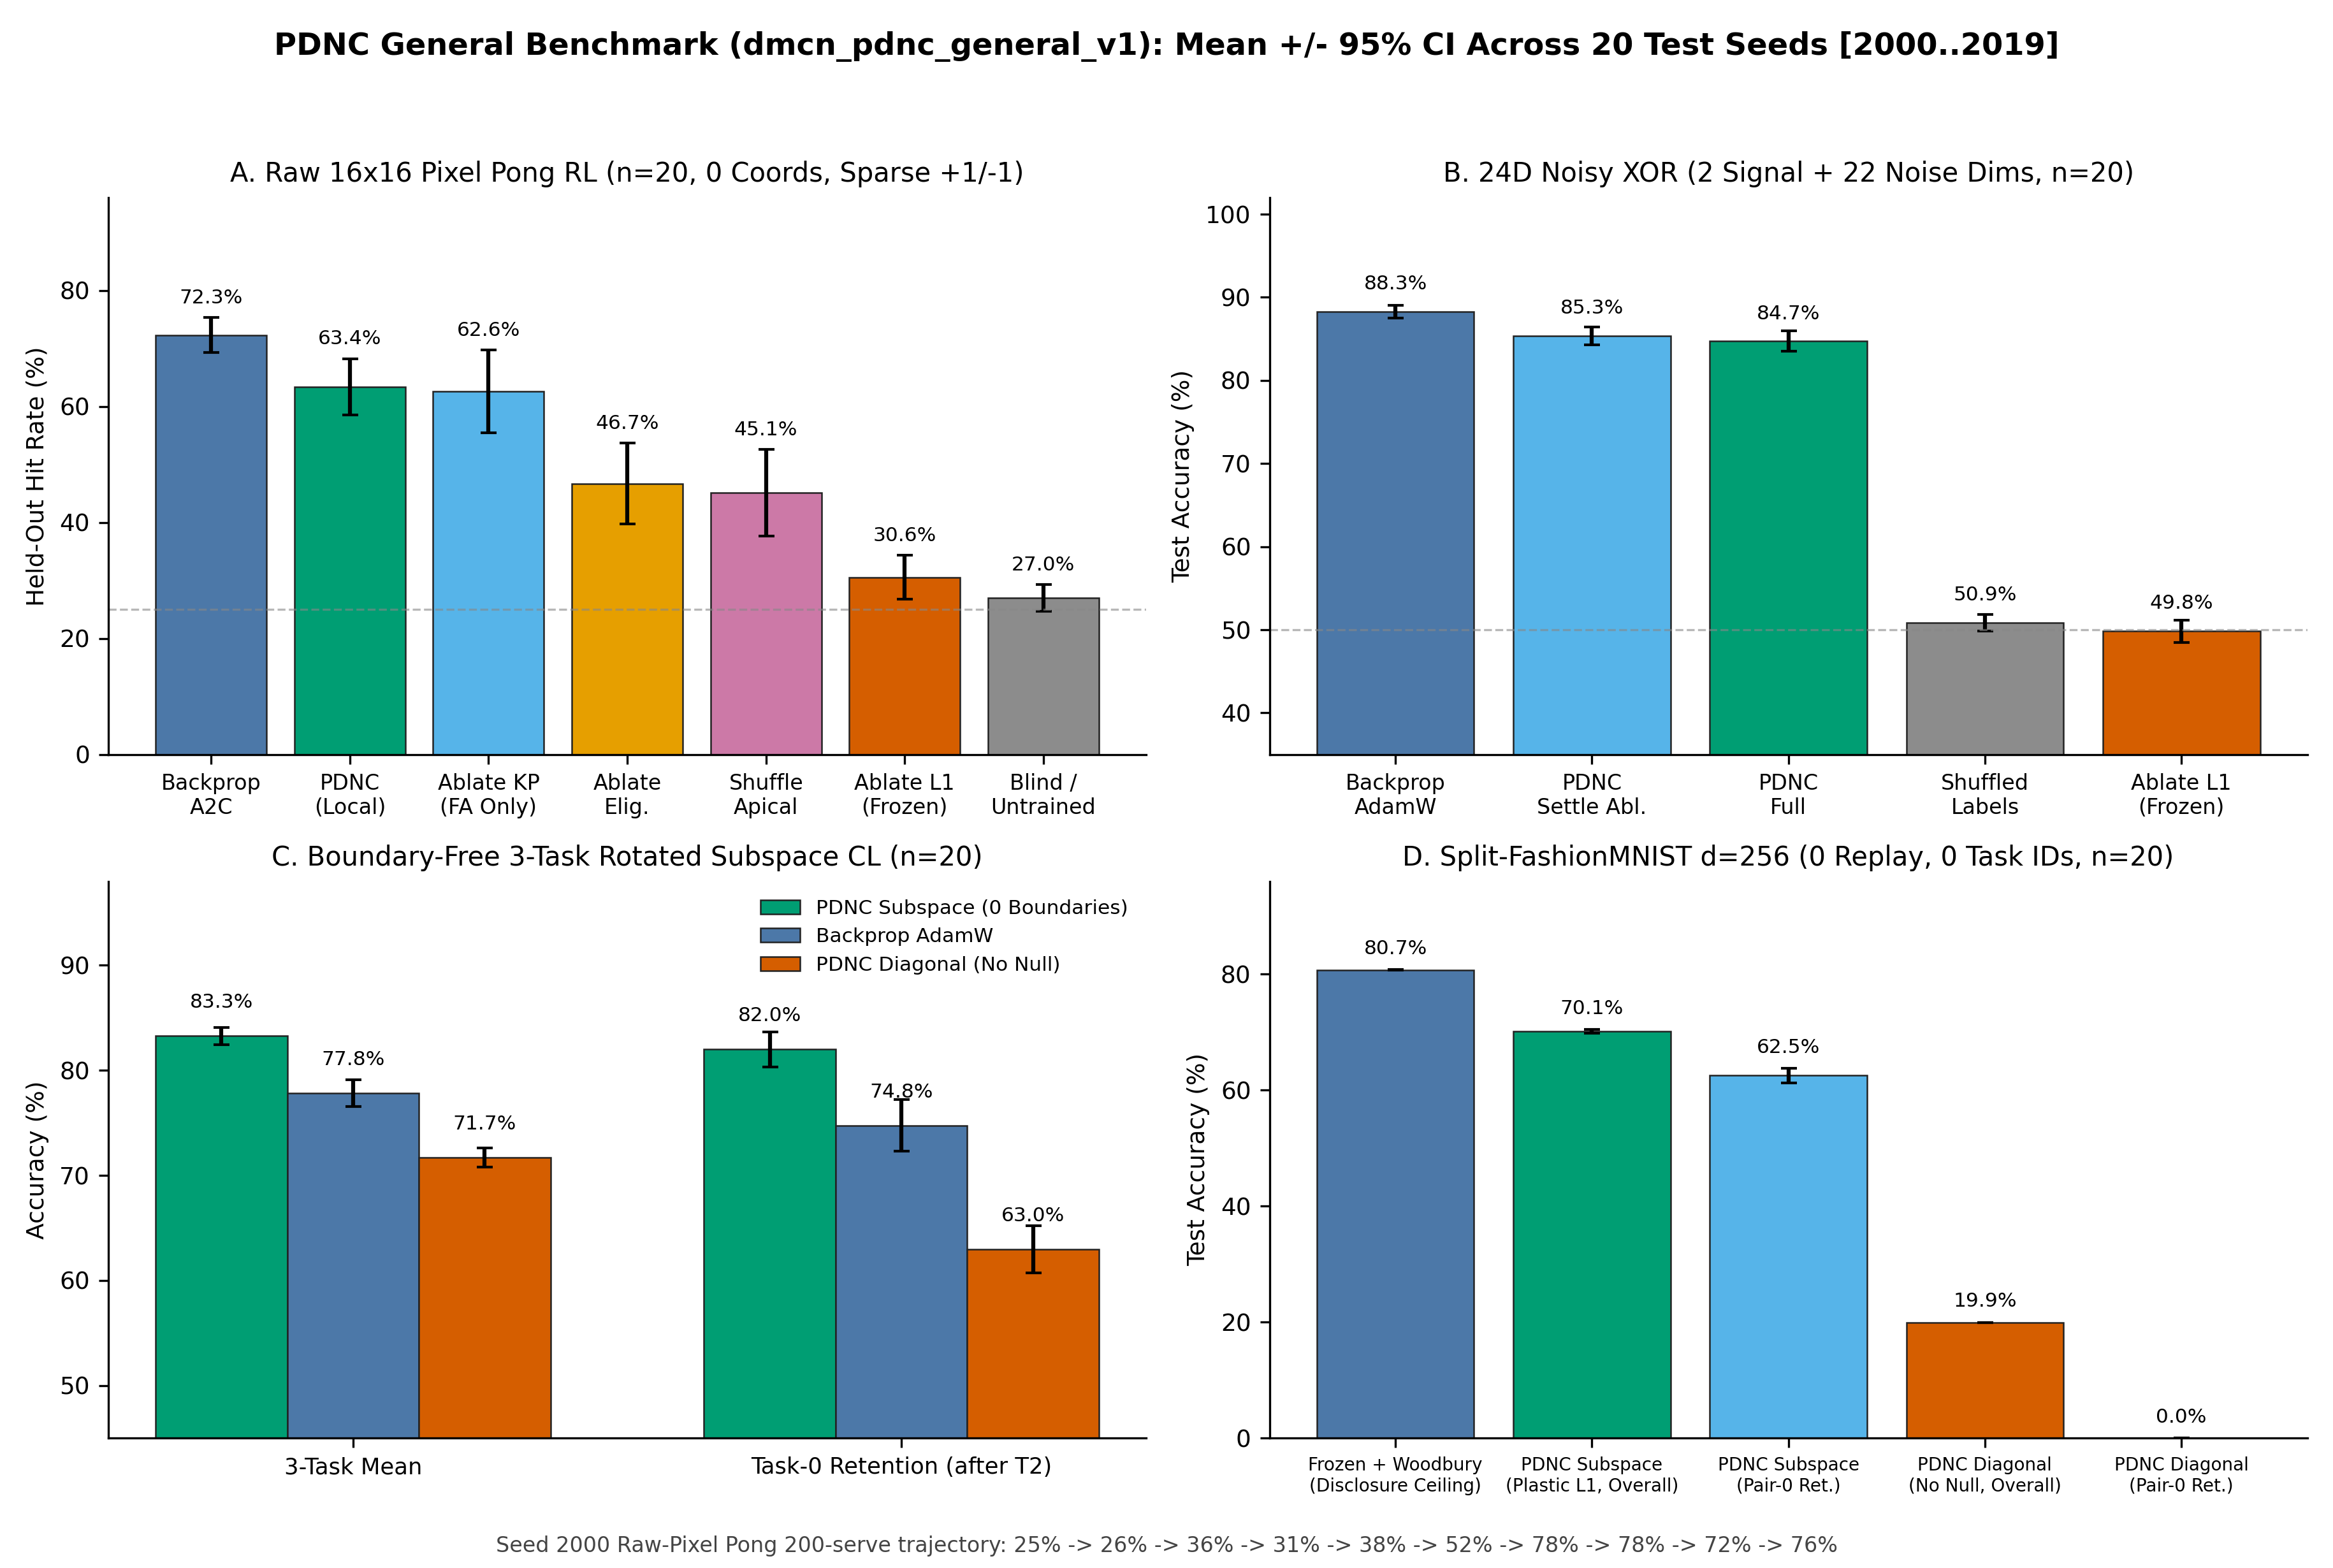
\includegraphics[width=0.98\linewidth]{fig11_pdnc_general.png}
    \caption{Dense \texttt{PDNC} across four tasks ($n=20$): Pixel Pong ($63.40\%$), 24D Noisy XOR ($84.71\%$), boundary-free rotated CL ($83.28\% > 77.85\%$ BP SGD), and \texttt{Split-FMNIST} showing L1 drift ($70.13\%$ vs.\ $80.72\%$ frozen).}
    \label{fig:pdnc}
\end{figure}

\begin{table}[htbp]
\centering
\caption{Raw $16\times 16$ Pixel Pong RL --- Dense vs.\ $4\times 4$ \texttt{Local-Patch PDNC} ($n=20$, $0$ Coords).}
\label{tab:pong}
\small
\resizebox{\linewidth}{!}{%
\begin{tabular}{@{}lrrrrl@{}}
\toprule
\textbf{Agent} & \textbf{L1 Syn.} & \textbf{ID Hit (\%)} & \textbf{SD} & \textbf{OOD Hit (\%)} & \textbf{Notes / Controls} \\
\midrule
\textbf{Local-Patch PDNC ($4\times 4$, 0 \texttt{.backward()})} & \textbf{4,851} & \textbf{$72.25 \pm 4.68$} & $10.69\%$ & $52.30 \pm 3.96$ & DirAlign $61.70\%$, KP cos $0.758$ ($+41.75\text{ pp} >$ Frozen) \\
Flat Backprop A2C (ref) & 65,536 & $72.30 \pm 3.05$ & $6.97\%$ & $49.70 \pm 2.90$ & Statistically tied ($-0.05\text{ pp}$) with $13.5\times$ more L1 \\
Local-Patch Backprop A2C ($4\times 4$) & 4,851 & $68.90 \pm 5.01$ & $11.42\%$ & --- & Local-Patch PDNC leads by $+3.35\text{ pp}$ \\
Dense Flat PDNC ($256\to 128$) & 65,664 & $63.40 \pm 4.84$ & $11.04\%$ & $47.65 \pm 3.94$ & KP cos $0.766$ (trailed Flat BP by $8.90\text{ pp}$) \\
Ablations ($-$Elig / ShufApical / Frozen) & 4,851 & $38.00 / 31.95 / 30.50$ & $7.63\text{--}12.31\%$ & --- & Proves eligibility + apical credit + L1 plasticity \\
Nulls (Untr / Blind / ShufRew / Rand) & --- & $27.05 / 25.20 / 24.55 / 22.15$ & $4.03\text{--}5.15\%$ & --- & All near random baseline \\
\bottomrule
\end{tabular}}
\end{table}

\subsection{Decentralized Swarms and Core Microcircuit Diagnostics}
Embedding $24$-branch spatial DMCN modules ($640$ FLOPs/step, $616$ bytes FP32 per boid) into $16$-boid Reynolds flocks (Figure~\ref{fig:swarm}, Table~\ref{tab:swarm}) beats a tuned Classical PID Disturbance Observer by $37.0\%$ on spatially varying wind ($3.97 \pm 0.87$ vs.\ $6.30 \pm 0.80$; Pure Boids $60.73$) and rescues $31.25\%$ blinded boids ($4.32$ vs.\ $22.54$ decoupled, $5.21\times$ lower error). We explicitly disclose that in Regimes~1--2, randomized neighbor headings (\texttt{Scrambled}: $2.19$, $3.07$) act as stabilizing velocity damping $-v_i$, isolating true consensus gains strictly to Regime~3. Table~\ref{tab:diag} summarizes the 7-task single-neuron microcircuit diagnostics ($100\%$ Causal XOR, $91.95\%$ Delayed XOR, $100\%$ 1-shot overwrite vs.\ $0\%$ Hebbian, $78.00\%$ 4-regime CL vs.\ $47.13\%$ BP SGD, $91.90\%$ T-Maze RL, and $92.32\%$ Kolen--Pollack $8\times 8$ digits).

\begin{figure}[htbp]
    \centering
    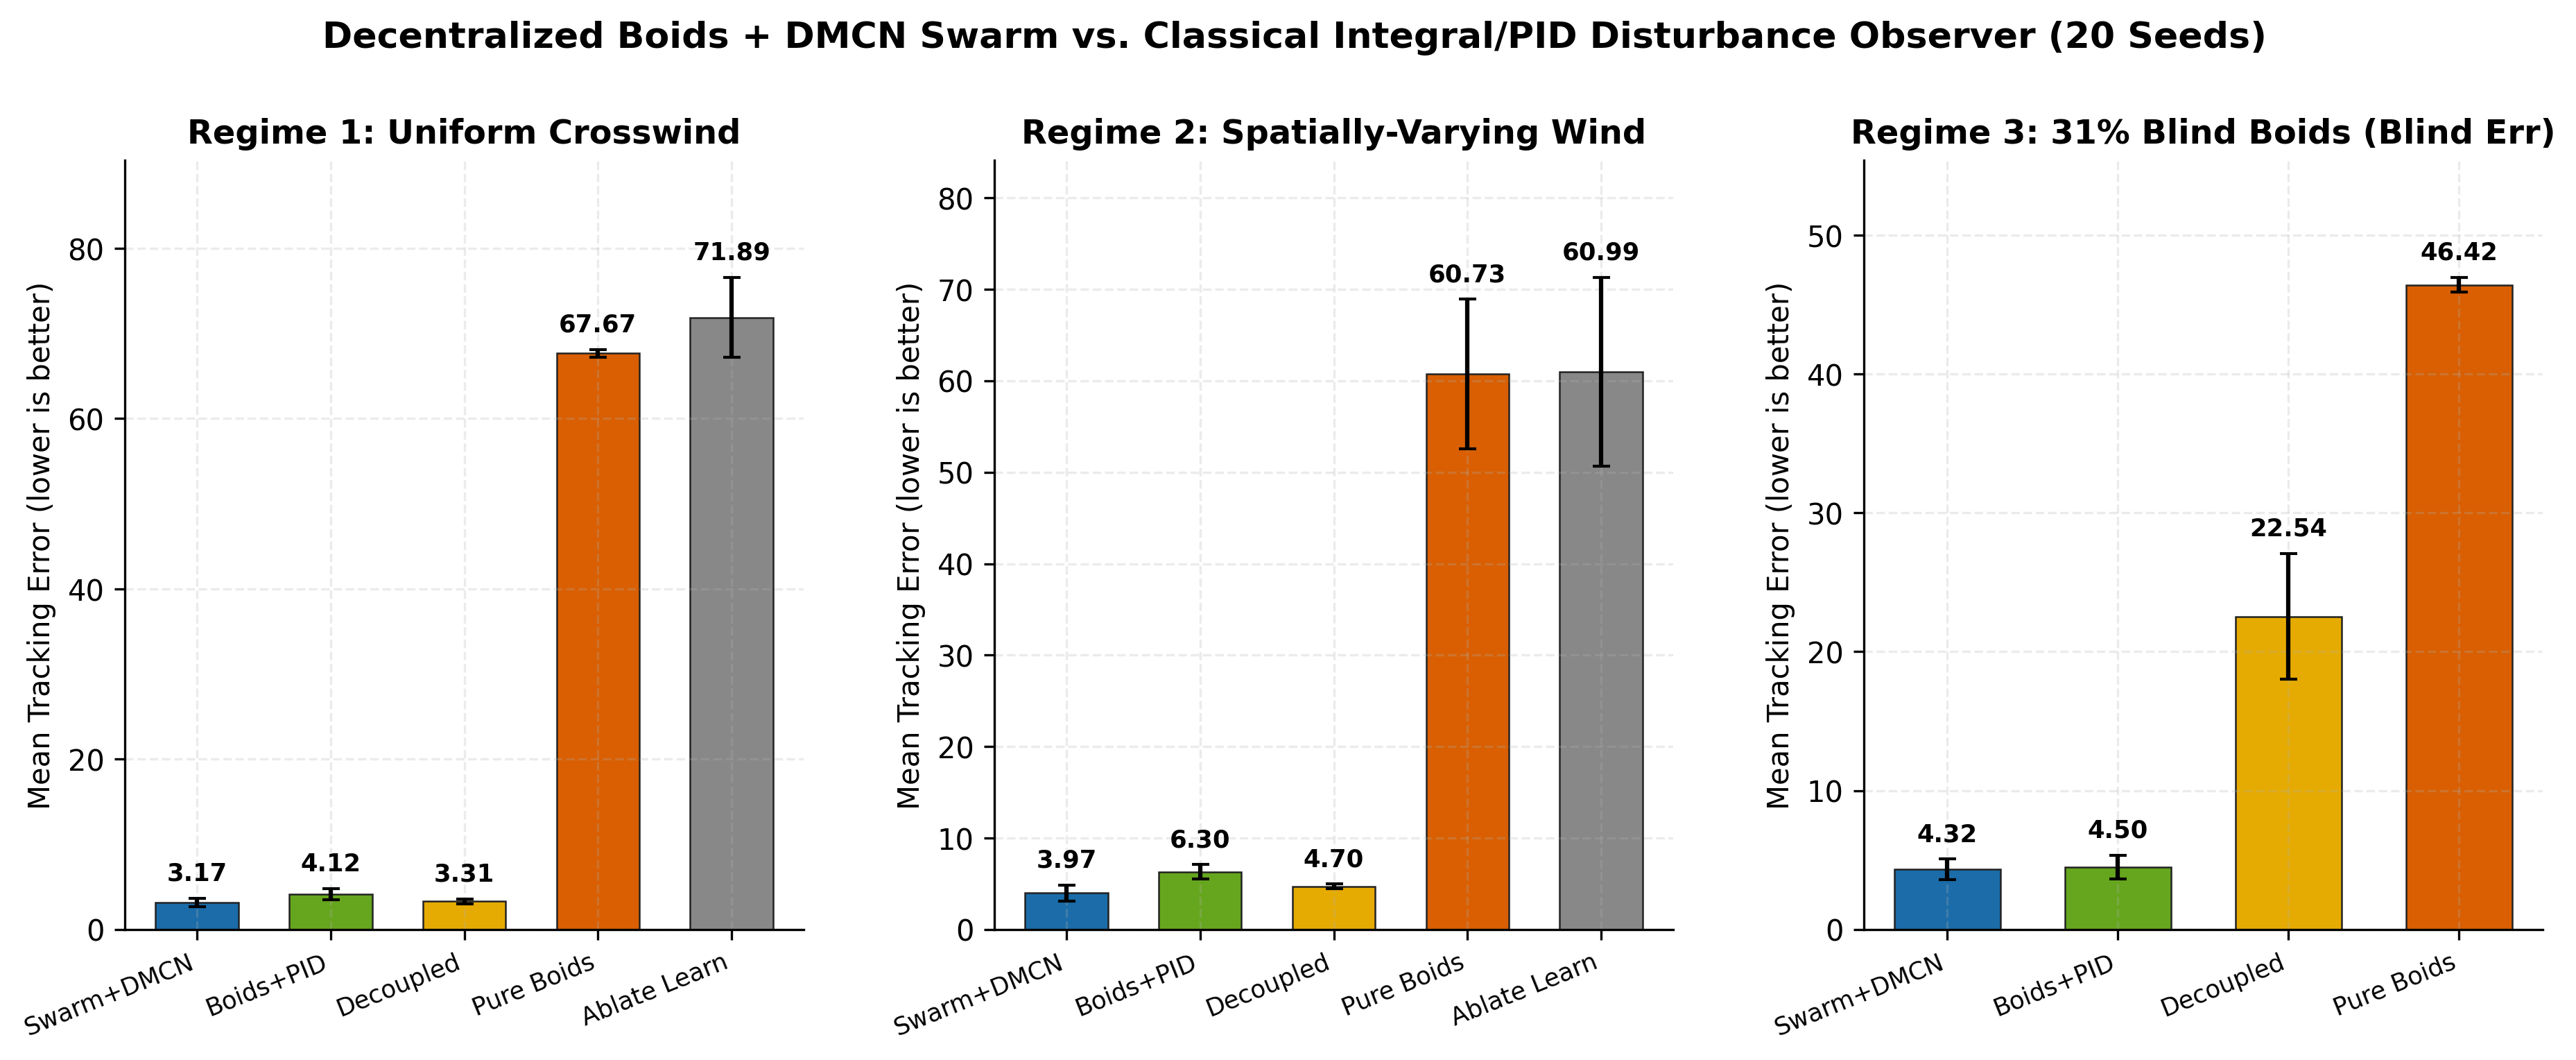
\includegraphics[width=0.98\linewidth]{fig4_swarm_boids_vs_pid.png}
    \caption{Decentralized 16-boid flock wind adaptation ($n=20$): DMCN cuts error by $37.0\%$ vs.\ PID under spatial wind and rescues $31.25\%$ blind agents ($4.32$ vs.\ $22.54$ decoupled).}
    \label{fig:swarm}
\end{figure}

\begin{table}[htbp]
\centering
\caption{Decentralized 16-Boid Wind Adaptation Tracking Error ($\downarrow$, $n=20$).}
\label{tab:swarm}
\small
\resizebox{\linewidth}{!}{%
\begin{tabular}{@{}lrrr@{}}
\toprule
\textbf{Controller / Control} & \textbf{Regime 1: Uniform Wind} & \textbf{Regime 2: Spatial Wind} & \textbf{Regime 3: 31\% Blind (Blind Err)} \\
\midrule
\textbf{Swarm + DMCN ($640$ FLOPs/boid)} & \textbf{$3.17 \pm 0.49$} & \textbf{$3.97 \pm 0.87$} ($-37.0\%$ vs PID) & $3.77 \pm 0.68$ (\textbf{Blind: $4.32 \pm 0.74$}) \\
Boids + Classical PID Observer & $4.12 \pm 0.63$ & $6.30 \pm 0.80$ & $4.19 \pm 0.81$ (Blind: $4.50 \pm 0.84$) \\
Pure Boids / EMA-Boids & $67.67$ / $67.10$ & $60.73$ / $59.40$ & $45.74$ / $45.32$ (Blind: $46.42$) \\
Null: \texttt{Decoupled} & $3.31 \pm 0.28$ & $4.70 \pm 0.28$ & $7.93 \pm 1.46$ (\textbf{Blind: $22.54 \pm 4.53$}) \\
Null: \texttt{Scrambled} \textit{(damping artifact)} & $2.19 \pm 0.16$ & $3.07 \pm 0.19$ & $3.51 \pm 0.25$ \\
\bottomrule
\end{tabular}}
\end{table}

\begin{table}[htbp]
\centering
\caption{Core Single-Neuron and Microcircuit Diagnostics ($n=20$, Zero \texttt{.backward()}).}
\label{tab:diag}
\small
\resizebox{\linewidth}{!}{%
\begin{tabular}{@{}lrrl@{}}
\toprule
\textbf{Diagnostic Task} & \textbf{DMCN Intact} & \textbf{Key Ablation / Baseline} & \textbf{Null Controls} \\
\midrule
Causal Noisy XOR & \textbf{$100.00\% \pm 0.00\%$} & No Non-Mono $76.63\%$, Logistic $49.63\%$, MLP $83.63\%$ & Untr $50.1\%$, Blind $49.5\%$, Shuf $52.0\%$ \\
Delayed Temporal XOR & \textbf{$91.95\% \pm 4.83\%$} & No Spine Traces $49.80\%$ & --- \\
1-Shot Recall + Overwrite & \textbf{$100.00\% \pm 0.00\%$} & No Fast Delta $9.38\%$, Hebbian Overwrite $0.00\%$ & Untr $0.0\%$, Blind $6.25\%$ \\
4-Regime Task-Free CL & \textbf{$78.00\% \pm 3.43\%$} & Single-Branch $50.63\%$, BP SGD $47.13\%$ & Untr $26.71\%$, Shuf $27.85\%$ \\
Lorenz + $10\times$ Shock \textit{(fixed homeo.)} & $0.3005 \pm 0.0618$ & No Homeo $0.2437$, BP MLP $0.3983$, NLMS $13.51$ & \textit{(Resolved by self-gate: $0.0054$)} \\
Delayed-Cue T-Maze RL & \textbf{$91.90\% \pm 8.70\%$} & No Spine $49.30\%$, REINFORCE $50.10\%$ & Blind $49.65\%$, ShufRew $49.45\%$ \\
$8\times 8$ Digits (Local KP) & \textbf{$92.32\% \pm 0.39\%$} & ShufApical $62.00\%$, SGD $92.15\%$, Adam $92.57\%$ & Untr $10.42\%$, Blind $10.03\%$, Shuf $9.44\%$ \\
\bottomrule
\end{tabular}}
\end{table}

\section{Negative Results, Limitations, and Open Problems}

Table~\ref{tab:failures} collects every refuted hypothesis, missed pre-registered bar, and open limit across the study.

\begin{table}[htbp]
\centering
\caption{Consolidated Ledger of Negative Results, Refutations, and Open Limitations.}
\label{tab:failures}
\footnotesize
\begin{tabular}{@{}p{4.0cm}p{4.4cm}p{5.8cm}@{}}
\toprule
\textbf{Experiment / Hypothesis} & \textbf{Observed Outcome ($n=20$)} & \textbf{Cause \& Scientific Takeaway} \\
\midrule
Unsupervised Motion-Oja Pixel L1 & \textbf{REFUTED:} $39.05\%$ vs.\ $45.30\%$ frozen L1 & Unrewarded k-WTA locked onto bright paddles and ignored ball. \\
Plastic L1 + Orthogonal Readout (FMNIST) & $70.13\%$ (\texttt{PDNC Subspace}) vs.\ $80.72\%$ frozen & L1 drift shifts hidden $H$, staling stored readout $P_2$. \\
\texttt{Local-Patch PDNC} vs.\ $74.0\%$ Bar & $72.25\% \pm 4.68\%$ (missed by $1.75\text{ pp}$, min $36.0\%$) & Tied Flat BP ($72.30\%$), but RL seed spread stays higher ($\text{SD}=10.69\%$). \\
Flat Dense \texttt{PDNC} on Pixel Pong & $63.40\%$ ($-8.90\text{ pp}$ vs.\ Flat BP) & Unstructured pixel fan-in weakens early KP alignment (fixed by $4\times 4$ patches). \\
Swarm \texttt{Scrambled} (Regimes 1--2) & $2.19$ / $3.07$ lower than DMCN $3.17$ / $3.97$ & Randomized neighbor headings act as velocity damping $-v_i$. \\
Memory \& Ternary Kernel Gaps & $O(d_\psi^2)$ Gram RAM; dense \texttt{torch.mm} execution & Continual L1 plasticity with $P_2$ and sparse bit-packed kernels remain open. \\
\bottomrule
\end{tabular}
\end{table}

Five concrete questions remain open: (1)~updating hidden weights $W_1$ while coherently rotating second-order readout curvature $P_2$ without replay; (2)~sub-quadratic curvature storage on wide heads without sacrificing eigenvalue-tail capacity; (3)~custom sparse bit-packed ternary CUDA or neuromorphic kernels; (4)~lowering worst-case RL seed variance under local feedback alignment; and (5)~extending local patch \texttt{PDNC} across deep natural-image hierarchies without pretrained front ends.

\section{Conclusion and Reproducibility}

DMCN and PDNC do not replace backpropagation for large-scale offline pretraining. Instead, they define concrete capabilities and boundaries for strictly local, replay-free computation: $90.32\% \pm 0.06\%$ under simultaneous blank delays, $50\times$ gain shocks, and sequential learning ($+21.6\text{ pp}$ to $+59.4\text{ pp}$ above \texttt{CausalRMS}-armed rivals); $68.65\% \pm 0.09\%$ on RGB \texttt{Split-CIFAR-100} ($0.0035\%$ from offline ridge, $2.62\times\text{--}3.86\times$ faster via Gram--Cholesky with $95\%$ sparse ternary encoders); $0.0054$ Lorenz chaos via causal self-gating; $99.58\%$ zero-shot rule binding; and $72.25\% \pm 4.68\%$ on raw pixel Pong RL tying Flat Backprop A2C using $13.5\times$ fewer Layer-1 synapses---while leaving continual hidden-feature drift and RL seed spread transparently open.

\textbf{Reproducibility Artifacts:} The PyTorch and NumPy implementation (\texttt{rpn/neuron\_v2/dmcn/}), benchmark suite (\texttt{rpn/benchmarks/}), unit tests (\texttt{rpn/tests/test\_dmcn.py}), pre-registrations, and frozen 20-seed JSON result archives (\texttt{results/}) accompany the repository.

\appendix
\section{Frozen Hyperparameter Configurations}
\begin{itemize}
    \item \textbf{Temporal Unified DMCN (\texttt{Split-MNIST}):} $d_{\text{in}}=112$, $K=5$ spine scales ($\tau \in \{28, 24, 20, 16, 14\}$, $\omega \in \{0, 0.52, 1.05, 1.57, 2.15\}$) $\Rightarrow d_\psi=1{,}232$; hidden expansion $2{,}048$ ($\tanh$, scale $2.0$, bias std $0.35$); readout ridge $5.0$, batch $256$, $1$ pass/pair. Block-diag: $4$ branches $\times 512$.
    \item \textbf{RGB \texttt{Split-CIFAR-100}:} Frozen \texttt{MobileNetV2} (\texttt{IMAGENET1K\_V1}) pooled $1280\text{-D}$ ($L_2$-normalized $\times\sqrt{1280}$), $[x, \tanh(Wx+b), 1]$ with $4{,}096$ dendritic units ($d_\psi=5{,}377$), ridge $20.0$, batch $256$, $1$ pass/task. Ternary density $0.05$. Baselines: \texttt{MLP (1280$\to$4096$\to$100)}, $10$ ep/task, \texttt{Adam lr=3e-4}, replay batch $256$; \texttt{Linear-RLS}: ridge $1.0$.
    \item \textbf{Self-Gating:} $32$ hidden units/pathway (\texttt{raw}, \texttt{homeo}, \texttt{spine}, \texttt{transient}), Hedge $\beta_{\text{gate}}=5.0$, loss EMA $0.06$, homeo EMA $0.05$, $\tau=2.5$, ridge $1.0$.
    \item \textbf{Compositional Binding:} $16$ Oja branches, top-$2$ winners, $\eta_{\text{oja}}=0.04$, soft $\ell_1$ $0.015$, ridge $0.1$ (\texttt{Color$\times$Shape}) / $0.05$ (\texttt{Rule$\times$Operand}).
    \item \textbf{$4\times 4$ Local-Patch \texttt{PDNC} (Pixel Pong):} $256$ pixels + transient ($\tau=2.0$, scale $1.5$) + bias ($513$ inputs), $4\times 4$ patches stride $2$, $3$ compartments/patch ($147$ units, $4{,}851$ L1 synapses), diagonal conditioning, $\eta=0.004$, Actor $0.003$, Critic $0.004$, $\gamma=0.95$, $\lambda=0.995$, $2{,}000$ train / $100$ ID + $100$ OOD eval serves.
\end{itemize}

\begin{thebibliography}{99}
\small
\bibitem{akrout2019} Akrout, M., Wilson, C., Humphreys, P., Lillicrap, T., \& Tweed, D.~B. (2019). Deep learning without weight transport. \textit{NeurIPS}, 32.
\bibitem{benna2016} Benna, M.~K., \& Fusi, S. (2016). Computational principles of synaptic memory consolidation. \textit{Nature Neuroscience}, 19(12), 1697--1706.
\bibitem{chaudhry2019} Chaudhry, A., Rohrbach, M., Elhoseiny, M., Ajanthan, T., Dokania, P.~K., Torr, P.~H.~S., \& Ranzato, M. (2019). On tiny episodic memories in continual learning. \textit{arXiv:1902.10486}.
\bibitem{gidon2020} Gidon, A., Zolnik, T.~A., Fidzinski, P., et al.\ (2020). Dendritic action potentials and computation in human layer 2/3 cortical neurons. \textit{Science}, 367(6473), 83--87.
\bibitem{kirkpatrick2017} Kirkpatrick, J., Pascanu, R., Rabinowitz, N., et al.\ (2017). Overcoming catastrophic forgetting in neural networks. \textit{PNAS}, 114(13), 3521--3526.
\bibitem{kolen1994} Kolen, J.~F., \& Pollack, J.~B. (1994). Backpropagation without weight transport. \textit{IEEE ICNN}, 3, 1375--1380.
\bibitem{larkum2013} Larkum, M. (2013). A cellular mechanism for cortical associations. \textit{Trends in Neurosciences}, 36(3), 141--151.
\bibitem{lillicrap2016} Lillicrap, T.~P., Cownden, D., Tweed, D.~B., \& Akerman, C.~J. (2016). Random synaptic feedback weights support error backpropagation for deep learning. \textit{Nature Communications}, 7, 13276.
\bibitem{mcdonnell2023} McDonnell, M.~D., Gong, D., Parvaneh, A., Abbasnejad, E., \& van den Hengel, A. (2023). RanPAC: Random projections and pre-trained models for continual learning. \textit{NeurIPS}, 36.
\bibitem{poirazi2003} Poirazi, P., Brannon, T., \& Mel, B.~W. (2003). Pyramidal neuron as two-layer neural network. \textit{Neuron}, 37(6), 989--999.
\bibitem{reynolds1987} Reynolds, C.~W. (1987). Flocks, herds, and schools: A distributed behavioral model. \textit{ACM SIGGRAPH}, 21(4), 25--34.
\bibitem{sandler2018} Sandler, M., Howard, A., Zhu, M., Zhmoginov, A., \& Chen, L.-C. (2018). MobileNetV2: Inverted residuals and linear bottlenecks. \textit{CVPR}, 4510--4520.
\bibitem{song2024} Song, Y., Millidge, B., Salvatori, T., Lukasiewicz, T., Xu, Z., \& Bogacz, R. (2024). Inferring neural activity before plasticity as a foundation for learning beyond backpropagation. \textit{Nature Neuroscience}, 27, 348--358.
\bibitem{vandeven2019} van de Ven, G.~M., \& Tolias, A.~S. (2019). Three scenarios for continual learning. \textit{arXiv:1904.07734}.
\bibitem{voelker2018} Voelker, A.~R., \& Eliasmith, C. (2018). Improving spiking dynamical networks: A Legendre memory unit. \textit{NeurIPS}, 31.
\bibitem{zhuang2022} Zhuang, H., Weng, Z., Wei, H., Xie, R., Toh, K.-A., \& Lin, Z. (2022). ACIL: Analytic class-incremental learning with absolute memorization and privacy protection. \textit{NeurIPS}, 35.
\end{thebibliography}

\end{document}
